\documentclass{llncs}

% \usepackage[a4paper, left=2.5cm, right=2.5cm]{geometry}
\usepackage{amsmath}
\usepackage{amsfonts}
\usepackage{amssymb}
\usepackage{mathrsfs}

% use float package to provide supprot for position option H (in figure env)
\usepackage{float}
\usepackage{afterpage}

\usepackage{tikz}
\usepackage{pgf}
\usepackage{reotex}
\usepackage{subfigure}
\usepackage{color}
\tikzset{
    state/.style={
           rectangle,
           rounded corners,
           draw=black, very thick,
           minimum height=2em,
           inner sep=2pt,
           text centered,
           },
}
\newcommand{\xy}[1]{\textcolor{red}{#1}}
\newcommand{\ly}[1]{\textcolor{blue}{#1}}
\newcommand{\sem}[1]{$[\![{#1}]\!]$}
% todo: what is the proper name of the new model ?
\newcommand{\nSTA}{\mbox{STA}_r}
\newcommand{\restrict}[2]{#1\restriction_{#2}}

\title{Capturing Stochastic and Real-Time Behavior in Reo Connectors}

\author{Yi Li, Xiyue Zhang, Yuanyi Ji and Meng Sun}
\institute{
    Department of Informatics and LMAM, School of Mathematical Sciences,\\
    Peking University\\
    \email{\{liyi\_math,zhangxiyue,jyy,sunm\}@pku.edu.cn}
}

\begin{document}
    \maketitle

    \begin{abstract}
Modern distributed systems are often coupled with flexible
architectures, composed of heterogenous components, and deployed on
different execution nodes. Under such frameworks, connectors (or
middlewares) are widely used to organize the separated components and
make them functioning. Apparently, reliability of such systems highly
depends on the correctness of their connectors. Reo is a channel-based
coordination language where complex connectors are constructed
from simpler ones in a compositional approach. In this paper, we
propose a stochastic and real-time extension of Reo, including a set
of new primitive channels and an expressive semantics named
\emph{Stochastic Timed Automata for Reo} ($\nSTA$). With the support
of $\nSTA$, different coordination scenarios in existing Reo
extensions can be easily encoded, integrated, and analyzed.
    \end{abstract}
    \begin{keywords}
    Coordination, Stochastic, Real-time, Distributed Systems
    \end{keywords}


    \section{Introduction}
\label{sec:intro}

Distributed systems have been booming everywhere in the past decades. On the one hand, Internet of Things (IoTs) are bringing network systems to daily life. Conventional devices are replaced by smart terminals, and in turn collected by central controller to construct `Smart Cities'. On the other hand, high-performance computation is being adapted from local workstations and clusters to cloud platform and elastic computation frameworks like Amazon EC2\cite{Newcombe2015} and Microsoft Azure\cite{Li2009}. These architectures are so popular that even small companies are starting to deploy their own private cloud systems. 

In modern systems, component-based method is widely used to speed up the development process. Long-tested functional units are encapuslated as \emph{components}, and get integrated in various systems through the \emph{connectors}. Under this developing model, a connector often implements the core software protocol, and consequently, suffers frequently from different kind of bugs.
Due to the distributed nature, it is really hard to have a bug-free connector designed manually. Unexpected scheduling and asynchronous clocks often lead to inconsistency, and on the other hand, unreliable connections and unstable delays make it even worse. A powerful framework is strongly required to formalize the connectors, and provided a basis for further formal analysis.

Reo\cite{ARBAB2004}, as one of the most popular coordination languages, was designed to formalize the hierachy and communication process between components. Based on channels and nodes, Reo provides a compositional approach where complex connectors are built from simpler ones.
In this paper, we extend Reo with new primitive channels and the enhanced semantics $\nSTA$, so that real-time and stochastic behavior can be easily handled.

Compared with existing timed and stochastic (or probabilistic) semantics of Reo \cite{Arbab2009,Baier2006,Meng2012,Meng2007}, our work provides a more powerful and universal solution. 
\begin{enumerate}
    \item \emph{Both timed behavior and stochastic behavior are supported, but declared separately.} This makes it free to model various coordination senarios by different combination patterns.
    \item \emph{Timelocks is avoided in this semantics, making the timed connectors fully implementable}. In the common semantics of timed Reo \cite{Arbab2006,Meng2012}, \emph{Timer} channels may get trapped in timelock, and in turn lead to unrealizable connectors.
\end{enumerate}

The paper is organized as follows. Section \ref{sec:reo} introduces Reo, the coordination language, and shows how we extend this language by adding new primitive channels. Then, in Section \ref{sec:semantics} we provide an adapted stochastic timed automata $\nSTA$ as its formal semantics. Section \ref{sec:casestudies} presents several examples. Related works and comparison are discussed in Section \ref{sec:discussion}. Finally, Section \ref{sec:conclusion} summarizes the paper and comes up with some future work we are going to work on.
    \section{Extending Reo for Stochastic and Timed Behavior}
\label{sec:reo}

\subsection{Reo}

Reo is a channel-based exogenous coordination language proposed by F. Arbab in \cite{ARBAB2004}, where concurrency protocols are manifested as \emph{connectors}. Basically, connectors are constructed in a compositional approach: complex ones are composed of simpler ones, where the atomic ones are called \emph{channels}. Channels are glued on \emph{nodes}, and they together perform the behavior of connectors.

\vspace{.5em}

\noindent\emph{Nodes.} There are three types of nodes in Reo: \emph{source nodes}, \emph{sink nodes} and \emph{mixed nodes}, as shown in Fig.~\ref{fig:typeofnodes}.

\begin{figure}[H]
    \centering
    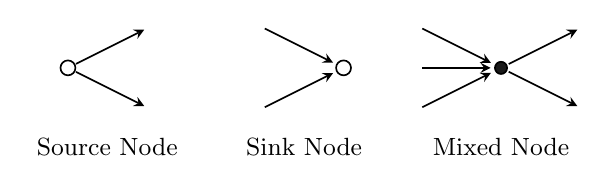
\begin{tikzpicture}[->,>=stealth',shorten >=1pt,auto,node distance=1.6cm,
  semithick]
    \tikzstyle{every node}=[font=\small]

    % source node
    \ionode{(P-1)}{(-4.5,0)}{}
    \sync{(P-1)}{(-3.5,0.5)}{}
    \sync{(P-1)}{(-3.5,-0.5)}{}

    \node (nt1) at (-4,-1) {Source Node};
    % sink node
    \ionode{(S-1)}{(-1,0)}{}
    \sync{(-2,0.5)}{(S-1)}{}
    \sync{(-2,-0.5)}{(S-1)}{}

    \node (nt2) at (-1.5,-1) {Sink Node};

    % mixed node
    \mixednode{(M-4)}{(1,0)}{}
    \sync{(0,0.5)}{(M-4)}{}
    \sync{(0,0)}{(M-4)}{}
    \sync{(0,-0.5)}{(M-4)}{}
    \sync{(M-4)}{(2,0.5)}{}
    \sync{(M-4)}{(2,-0.5)}{}

    \node (nt3) at (1,-1) {Mixed Node};

\end{tikzpicture}
    \caption{Three Types of Nodes}
    \label{fig:typeofnodes}
\end{figure}

Essentially, a \emph{source node} performs \emph{replicate} behavior. That is, any coming data values will be broadcasted sychronously if and only if all its successors are ready to accept. A \emph{sink node} performs \emph{merge} behavior, accepting data values from its predecessors one at a time (this can be a non-deteministic choice if all predecessors are ready to write). And a \emph{mixed node}, literally, performs both behavior at the same time, randomly picking one input and broadcast it to all outputs.

\vspace{.5em}
\noindent\emph{Channels.} As the basic functional units in Reo, channels are supposed to describe basic coordination behavior among \emph{channel ends}. Channel ends can be either a \emph{source end} or a \emph{sink end}, indicating the direction of data flow. A set of primitive channels can be found in Fig.~\ref{fig:basicchannels}, where we use arrows to indicate the type of channel ends.

\begin{figure}[H]
    \centering
    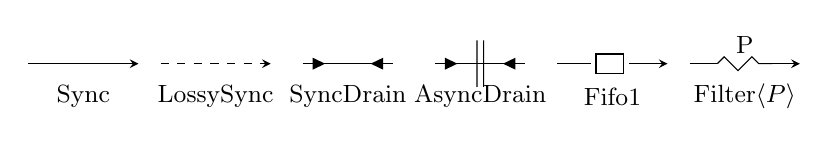
\begin{tikzpicture}[scale=1.4]

\tikzstyle{every node}=[font=\small]
\tikzstyle{label}=[draw=none]

\draw (0.5, -0.3) node[label] {Sync};
\draw (1.7, -0.3) node[label] {LossySync};
\draw (2.9, -0.3) node[label] {SyncDrain};
\draw (4.1, -0.3) node[label] {AsyncDrain};
\draw (5.3, -0.3) node[label] {Fifo1};
\draw (6.5, -0.3) node[label] {Filter$\langle P\rangle$};

\sync{(0,0)}{(1,0)}{}
\lossysync{(1.2,0)}{(2.2,0)}{}
\syncdrain{(2.4,0)}{(3.4,0)}{}
\asyncdrain{(3.6,0)}{(4.6,0)}{}
\fifoe{(4.8,0)}{(5.8,0)}{}
\filter{(6.0, 0)}{(7.0, 0)}{node[above] {P}}

\end{tikzpicture}
    \caption{Primitive Channels}
    \label{fig:basicchannels}
\end{figure}

Channels can be either \emph{synchronous} or \emph{asynchronous}. A channel is \emph{synchronous} if and only if the read and write operations on its channel ends are always performed simultaneously. The behavior of some primitive channels are specified as follows.

\begin{description}
    \item \emph{Sync(A:source,B:sink)} is a \emph{synchronous} channel that delivers data values from its source end $A$ to its sink end $B$. A synchronous channel is fired only when $A$ is prepared for reading and $B$ is ready for writing. 
    \item \emph{LossySync(A:source,B:sink)}
    is an \emph{input-enabled synchronous} channel with a source end $A$ and a sink end $B$. Such channels are always prepared to accept data from $A$. However, the transmission process could be unreliable. If $B$ is also ready for writing, the received value will be sent to $B$. Otherwise the value will be dropped immediately.
    \item \emph{SyncDrain(A\:B:source)} is a \emph{synchronous} channel with two source ends $A$ and $B$. It only accepts input from both $A$ and $B$ simultaneously and drop them together after being received.
    \item \emph{AsyncDrain(A\:B:source)} is an asynchronous variation of \emph{SyncDrain}. The most important difference is that it accepts data only from one end at a time. If both ends are ready to read, one of them (randomly picked) should wait.
    \item \emph{FIFO1(A:source,B:sink)} is an asynchronous channel with a source end $A$ and a sink end $B$. A FIFO1 channel can temporarily store one data value from its source end $A$ for arbitrary duration, and deliver it anytime when $B$ is ready to write. When the buffer is full, a FIFO1 cannot accept any more data values.
    \item \emph{Filter$\langle P\rangle$(A:source,B:sink)}
    is a synchronous channel with a source end $A$, a sink end $B$ and a boolean function $P$ as its parameter. When there is data at end A, first we have to check if the value satisfies the filter predicate $P$. If the answer is yes, the channel will behave just as \emph{Sync}, otherwise the value will be simply dropped.
\end{description}

\noindent\emph{Composition.} Formalization of nodes sometimes becomes rather complicated, as arbitrary number of incoming and outgoing edges may be involved. Usually, we tend to introduce two ternary channels \emph{Replicator}, \emph{Merger} and use their combinations to capture the behavior of mixed nodes.

\begin{figure}[H]
    \centering
    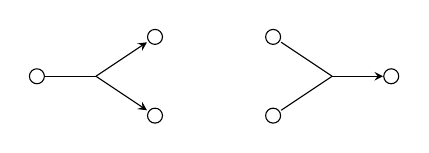
\begin{tikzpicture}
    % replicator
    \ionode{(P-1)}{(0,0)}{}
    \ionode{(P-2)}{(1.5,0.5)}{}
    \ionode{(P-3)}{(1.5,-0.5)}{}
    \sync*{(P-1)}{(0.75,0)}{}
    \sync{(0.75,0)}{(P-2)}{}
    \sync{(0.75,0)}{(P-3)}{}

    \ionode{(M-1)}{(3,0.5)}{}
    \ionode{(M-2)}{(3,-0.5)}{}
    \ionode{(M-3)}{(4.5,0)}{}
    \sync*{(M-1)}{(3.75,0)}{}
    \sync*{(M-2)}{(3.75,0)}{}
    \sync{(3.75,0)}{(M-3)}{}
\end{tikzpicture}
    \caption{Replicator and Merger}
\end{figure}

\begin{description}
    \item \emph{Replicator(A:source,B\:C:sink)} is a \emph{synchronous} broadcast channel with a source end $A$ and two sink ends $B,C$. The channel accepts data values from $A$, and broadcast them to $B,C$ iff. both $B$ and $C$ are ready to write.
    \item \emph{Merger(A\:B:source,C:sink)}
    is an \emph{asynchronous} channel that collects inputs from either $A$ or $B$ and send them to $C$ simultaneously if $C$ is prepared.
\end{description}

\emph{Replicator}s and \emph{Merger}s can reduce the number of incoming and outgoing edges for mixed nodes. For example, if we replace two outgoing edges with a \emph{Replicator} channel, the number of edges would be reduced by 1. After a finite number of replacements, all the mixed nodes can be simplified as nodes with one incoming edge and one outgoing edge, which is called \emph{flow-through}.
When processing the semantics of connectors, we assume that all the mixed nodes are \emph{flow-through} ones. However, to make it easy to understand, in the figures we still draw the mixed nodes in its original form.

\subsection{Capturing Timed and Stochastic Behavior}

In this subsection, we come up with some new primitive channels, which extend Reo and make it capable to specify timed and stochastic behavior.
Compared with other formal languages, Reo provides a framework which can be easily extended by adding new channel types to the primitive channel set. Usually, new channels should be simple enough, and orthogonal to the existing ones. Following this idea, here we propose three channel types, capturing \emph{data evolution}, \emph{stochastic choice}, and \emph{timed delay}.

\begin{figure}[t]
    \centering
    \label{fig:newchannels}
    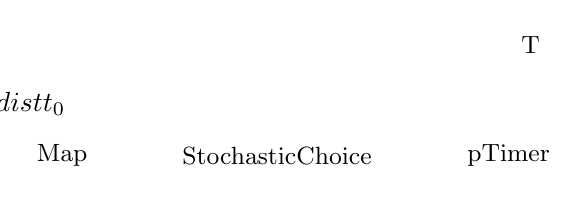
\begin{tikzpicture}[scale=1.4]

\tikzstyle{every node}=[font=\small]
\tikzstyle{label}=[draw=none]

\draw (0.75, -0.4) node[label] {Map};
\draw (2.7, -0.4) node[label] {StochasticChoice};
\draw (4.8, -0.4) node[label] {pTimer};

\draw (5, 0.6) node[label] {T};

\map{(0,0)}{(1.5,0)}{node [above=3] {$f$}}
\choice{(1.95,0)}{(3.45,0)}{node [above=0.2cm, xshift=-0.6cm] {$dist$}}
\ptimer{(4.1,0)}{(4.85, 0.6)}{(5.6,0)}{node [above=1, xshift=-0.2cm] {$t_0$}}

\end{tikzpicture}
    \caption{Extended Primitive Channels}
\end{figure}

\begin{description}
    \item \emph{Map$\langle f\rangle$(A:source,B:sink)}
        is a synchronous channel with a source end $A$, a sink end $B$ and a mapping function $f$ as its parameter. The function $f$ has exactly one argument. However, the argument may not always be used (for example, the function can be constant, i.e. $f(\cdot)=1$).
        A \emph{Map} channel behaves similar to a \emph{Sync} channel. But it will apply $f$ to all the incoming data values and write the results to $B$.
    \item \emph{StochasticChoice$\langle dist\rangle($A:source,B:sink)} is a combination of a $Sync$ channel and a randomizer.
        It accepts data values from source node $A$ only when $B$ is writable. Then, a random value following distribution $dist$ will be sent to $B$, where $dist$ is provided as a parameter.
    \item \emph{pTimer$\langle t_0\rangle$(A\:T:source,B:sink)} is a \emph{parameterized} version of $t$-Timer in \cite{Meng2012}. 
        The channel accepts a data value from $A$ and throw out a timeout signal to $B$ after a certain delay. The delay is initialized by $t_0$, and can be rewritten by values coming from the source end $T$. Initially, a \emph{pTimer} channel is ready to accept a numeric value from $T$ and resets its timeout as that value. However, after the channel accepts a data value from $A$ and start counting, any new value from $T$ will reset the \emph{pTimer}, force it jumping to the initial state and forget the current counting status. If the counting process is not terminated by $T$, it will finish after the delay. Then a timeout signal will be sent to $B$ if it is writable, or simply ignored otherwise.

\end{description}



    \section{Stochastic Timed Automata for Reo}
\label{sec:semantics}

In this section, first we introduce the formal model $\nSTA$ that yields the basis for reasoning about timed and stochastic behavior of connectors. Then we define the new semantics for primitive Reo channels based on $\nSTA$, and explain how to construct the $\nSTA$ for complex connectors by applying the \emph{product} and \emph{hiding} operators to the $\nSTA$ for simpler ones.
\subsection{$\nSTA$}

Stochastic timed automata (STA) \cite{HahnHH14} is a powerful formalism to describe stochastic behavior and real-time behavior. Both continuous distribution and discrete distribution are supported in STA. In this paper, we slightly adapt STA as $\nSTA$ so that Reo channels can be depicted more naturally and clearly.
Before touching the technical details of $\nSTA$, we first introduce some notations that will be used later.

During the rest of this paper, we will use $\mathbb{D}$ to denote the \emph{data scope}, which can be any finite set, the set of real numbers $\mathbb{R}$ or their union. Namely, $\mathbb{D}$ is finite, or $\mathbb{R}\subseteq \mathbb{D}$ and $\mathbb{D}\backslash \mathbb{R}$ is finite. When the data scope is limited to finite sets, stochastic assignments are, obviously, not supported. For example, if $\mathbb{D}=\{1,2\}$, $v:=norm(e,\sigma)$ is an invalid assignment while $v':=1+\operatorname{B}(1, 0.5)$ is acceptable, where $norm$ and $\operatorname{B}$ stand for normal and binomial distribution respectively. We use $Dist(S)$ to denote the set of continuous or discrete distributions on $S$.

\begin{definition}[Evaluations]
Suppose $V$ is a finite set of variables, an \emph{evaluation} on $V$ is defined as a function $ev_V:V\rightarrow \mathbb{D}$ that maps a variable identifier to a value. Similarly, we can also define clock evaluations on $C$ as $ev_C:C\rightarrow \mathbb{R}$, where $C$ is a set of clock variables. Natually, we can use $EV_V$ to denote the set of all evaluations on $V$, $EV_C$ to denote the set of all clock evaluations on $C$, and $EV$ to denote their combination, i.e. 

\begin{displaymath}
    EV=\Bigg\{ev:V\cup C\rightarrow \mathbb{D}\cup\mathbb{R}|
    ev(v)=
    \left\{
        \begin{array}{lr}
            ev_v(v) & v\in V \\
            ev_c(v) & v\in C
        \end{array}
    \right.
    , ev_v\in EV_V, ev_c\in EV_C
    \Bigg\}
\end{displaymath}

\end{definition}

In practice, evaluations are usually represented by a set of assignment statements. E.g., \emph{\{a := TIMEOUT, b := 1, c := 0.5, $\cdots$\}}.

In $\nSTA$, there is a very different concept named \emph{adjoint variable}. That is, for each external action $A$, when it shows up, there must be a data value coming along, and assigned to its adjoint variable \emph{dA}. Adjoint variables are used to describe the channels' behavior : channel ends are triggered if and only if a data value comes (or leaves).

\begin{definition}[$\nSTA$]
Stochastic Timed Automata for Reo ($\nSTA$) is defined as an 8-tuple $\langle L, l_0, Acts, V, V_0, C, Inv, E\rangle$ where:

\begin{itemize}
    \item $L$ is a finite set of locations,
    \item $l_0\in L$ is an initial location,
    \item $Acts$ is a finite set of actions with the internal action $i\in Acts$ (we use $Acts_e$ to denote the set of external actions $Acts\backslash \{i\}$),
    \item $V$ is a finite set of variables that satisfies $\forall A\in Acts_e, dA\in V$,
    \item $V_0\in EV$ is an initialized function for variables,
    \item $C$ is a finite set of clocks (we always assume that $V\cap C=\varnothing$),
    \item $Inv:L\rightarrow (EV\rightarrow Bool)$ is a function that maps locations to their corresponding invariants,
    \item $E$ is a finite set of edges. An \emph{edge} of a $\nSTA$ is defined as a 5-tuple $\langle l, acts, g, u, l'\rangle$ where
        \begin{itemize}
            \item $l\in L$ is the source location,
            \item $acts\in P(Acts_e)\cup\{\{i\}\}$ is a set of actions (external actions and internal actions do not appear on the same edge simultaneously). The transition can be fired either $acts=\{i\}$ or all external actions in $acts$ are prepared,
            \item $g:EV\rightarrow Bool$ is the guard constraint that maps an evaluation (for both variables and clocks) to a boolean value \emph{true} or \emph{false},
            \item $u:EV\rightarrow Dist(EV)$ is a random assignment that updates the current evaluation with a random sample following a certain distribution of $Dist(EV)$,
            \item $l'\in L$ is the target location.
        \end{itemize}
\end{itemize}
\end{definition}

In the following, we write $l \xrightarrow{\textbf{acts}, g, u}_E l'$ instead of $\langle l, acts, g , u, l' \rangle \in E$, or simply $l \xrightarrow{\textbf{acts}, g, u} l'$ under ambiguity-free context. Meanwhile, in a $\nSTA$ graph we use [\textbf{acts}, \emph{g}]\emph{u} to label such a transition (see in Fig.~\ref{fig:basic}).

\subsection{Semantics of Primitive Channels}
As mentioned before, $\nSTA$ for a given Reo connector is constructed in a compositional way. In this subsection, we provide semantics of the primitive channels as $\nSTA$, including both original and extended ones. The \sem{\cdot} operator is used to denote \emph{semantics map} which maps a Reo connector to its semantics as $\nSTA$.

\begin{figure}[H]
    \centering
    \resizebox{\textwidth}{!}{
        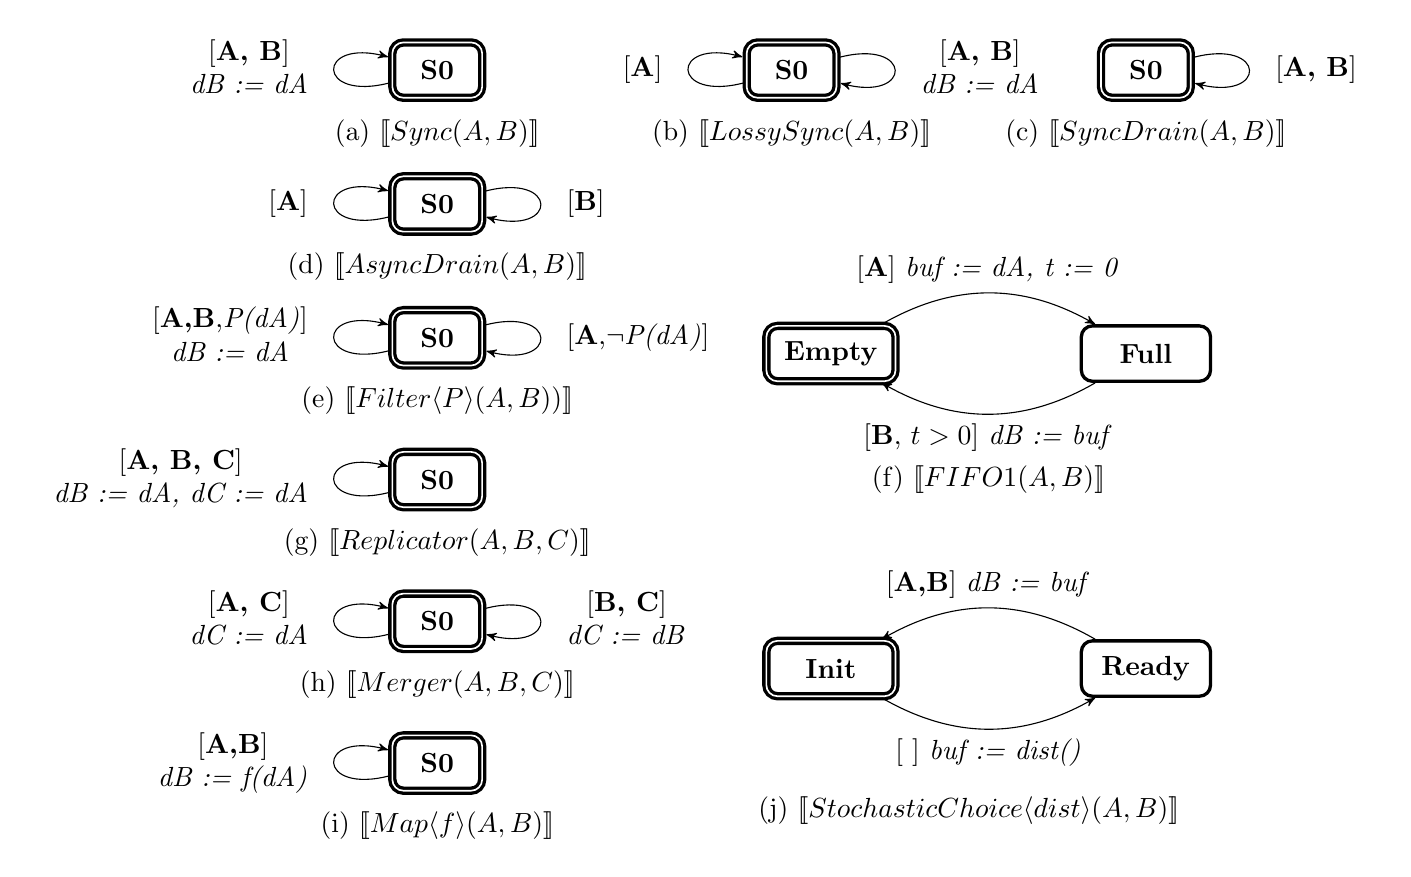
\begin{tikzpicture}[>=stealth']

    % ------------------------------- SYNC & LOSSY ---------------------------------
    % State: ACK with different content
    \node[state, double,   	% layout (defined above)
    text width=1cm, 	% max text width    
    anchor=center] (S0) 	% posistion relative to the center of the 'box'
    {\textbf{S0}};

    \node[state, double,   	% layout (defined above)
    text width=1cm, 	% max text width
    right of=S0,
    node distance=4.5cm,    
    anchor=center] (SL0) 	% posistion relative to the center of the 'box'
    {\textbf{S0}};

    \node[below of=S0, node distance=0.8cm] {(a) \sem{Sync(A, B)}};
    \node[below of=SL0, node distance=0.8cm] {(b) \sem{LossySync(A, B)}};
    
    % draw the paths and and print some Text below/above the graph
    \path (S0)  edge[loop left] node{
        \begin{tabular}{c}
            [\textbf{A, B}] \\
            \emph{dB := dA}
        \end{tabular}
    } (S0);

    \path (SL0)  edge[loop right] node{
        \begin{tabular}{c}
            [\textbf{A, B}] \\
            \emph{dB := dA}
        \end{tabular}
    } (SL0)

    (SL0) edge[loop left] node{
        \begin{tabular}{c}
            [\textbf{A}]
        \end{tabular}
    } (SL0)
    ;

    % ------------------------------- DRAINS ---------------------------------

    % State: ACK with different content
    \node[state, double,   	% layout (defined above)
    text width=1cm, 	% max text width
    right of=SL0,
    node distance=4.5cm,
    anchor=center] (SD0) 	% posistion relative to the center of the 'box'
    {\textbf{S0}};

    \node[state, double,   	% layout (defined above)
    text width=1cm, 	% max text width
    below of=S0,
    node distance=1.7cm,    
    anchor=center] (ASD0) 	% posistion relative to the center of the 'box'
    {\textbf{S0}};

    \node[below of=SD0, node distance=0.8cm] {(c) \sem{SyncDrain(A,B)}};
    \node[below of=ASD0, node distance=0.8cm] {(d) \sem{AsyncDrain(A,B)}};
    
    % draw the paths and and print some Text below/above the graph
    \path (SD0)  edge[loop right] node{
        \begin{tabular}{c}
            [\textbf{A, B}]
        \end{tabular}
    } (SD0);

    \path (ASD0)  edge[loop right] node{
        \begin{tabular}{c}
            [\textbf{B}]
        \end{tabular}
    } (ASD0)

    (ASD0) edge[loop left] node{
        \begin{tabular}{c}
            [\textbf{A}]
        \end{tabular}
    } (ASD0)
    ;

    % ------------------------------- FILT ---------------------------------

    \node[state, double,   	% layout (defined above)
    text width=1cm, 	% max text width
    below of=ASD0,
    node distance=1.7cm,    
    anchor=center] (F0) 	% posistion relative to the center of the 'box'
    {\textbf{S0}};


    \path (F0)  edge[loop right] node{
        \begin{tabular}{c}
            [\textbf{A},\emph{$\lnot$P(dA)}]
        \end{tabular}
    } (F0)

    (F0) edge[loop left] node{
        \begin{tabular}{c}
            [\textbf{A,B},\emph{P(dA)}] \\
            \emph{dB := dA}
        \end{tabular}
    } (F0)
    ;

    % ------------------------------- FIFO ---------------------------------
    \node[state,    	% layout (defined above)
    text width=1.5cm, 	% max text width
    below of=SD0,
    node distance=3.6cm,
    anchor=center] (ready) 	% posistion relative to the center of the 'box'
    {\textbf{Full}};

    \node[state, double,   	% layout (defined above)
    text width=1.5cm, 	% max text width    
    left of=ready,
    node distance=4cm,
    anchor=center] (init) 	% posistion relative to the center of the 'box'
    {\textbf{Empty}};

    \node[below of=F0, node distance=.8cm] {(e) \sem{Filter\langle P\rangle(A,B))}};
    \node[below of=init, node distance=1.6cm,xshift=2cm] {(f) \sem{FIFO1(A,B)}};
    
    % draw the paths and and print some Text below/above the graph
    \path
        (ready)   edge[bend left, ->]
            node[below] {[\textbf{B}, $t > 0$] \emph{dB := buf}} 
        (init)

        (init)  edge[bend left, ->]
            node[above] {[\textbf{A}] \emph{buf := dA, t := 0}} 
        (ready);

    % replicator
    \node[state, double,   	% layout (defined above)
    text width=1cm, 	% max text width
    below of=F0, 
    node distance=1.8cm,   
    anchor=center] (REP0) 	% posistion relative to the center of the 'box'
    {\textbf{S0}};

    % draw the paths and and print some Text below/above the graph
    \path (REP0)  edge[loop left] node{
        \begin{tabular}{c}
            [\textbf{A, B, C}] \\
			\emph{dB := dA, dC := dA}
        \end{tabular}
    } (REP0);

    \node[state, double,   	% layout (defined above)
    text width=1cm, 	% max text width
    below of=REP0,
    node distance=1.8cm,    
    anchor=center] (MRG0) 	% posistion relative to the center of the 'box'
    {\textbf{S0}};

    \path (MRG0)  edge[loop right] node{
        \begin{tabular}{c}
            [\textbf{B, C}] \\
            \emph{dC := dB}
        \end{tabular}
    } (MRG0)

    (MRG0) edge[loop left] node{
        \begin{tabular}{c}
            [\textbf{A, C}] \\
            \emph{dC := dA}
        \end{tabular}
    } (MRG0)
    ;

    \node[below of=REP0, node distance=0.8cm] {(g) \sem{Replicator(A,B,C)}};
    \node[below of=MRG0, node distance=0.8cm] {(h) \sem{Merger(A,B,C)}};

    % State: ACK with different content
    \node[state, double,   	% layout (defined above)
    text width=1cm, 	% max text width    
    below of=MRG0,
    node distance=1.8cm,
    anchor=center] (MAP0) 	% posistion relative to the center of the 'box'
    {\textbf{S0}};
    
    % draw the paths and and print some Text below/above the graph
    \path (MAP0)  edge[loop left] node{
        \begin{tabular}{c}
            [\textbf{A,B}] \\
            \emph{dB := f(dA)}
        \end{tabular}
    } (MAP0);

    \node[below of=MAP0, node distance=0.8cm] {(i) \sem{Map\langle f\rangle(A,B)}};

    % stochastic choice
    \node[state, double,   	% layout (defined above)
    below of=init,
    node distance=4cm,
    text width=1.5cm, 	% max text width    
    anchor=center] (sinit) 	% posistion relative to the center of the 'box'
    {\textbf{Init}};
    
    \node[state,    	% layout (defined above)
    text width=1.5cm, 	% max text width
    right of=sinit,
    node distance=4cm,
    anchor=center] (sready) 	% posistion relative to the center of the 'box'
    {\textbf{Ready}};

    \node[below of=sinit, node distance=1.8cm, xshift=1.75cm] {(j) \sem{StochasticChoice\langle dist\rangle(A,B)}};
    
    
    % draw the paths and and print some Text below/above the graph
    \path
        (sinit)   edge[bend right, ->] 
            node[below] {[ ] \emph{buf := dist()}} 
        (sready)

        (sready)  edge[bend right, ->]
            node[above] {[\textbf{A,B}] \emph{dB := buf}} 
        (sinit);

\end{tikzpicture}
    }
    \caption{Semantics of Primitive Channels}
    \label{fig:basic}
\end{figure}


\begin{description}
    \item[\sem{Sync(A, B)}] in Fig.~\ref{fig:basic}(a) has only one single location and a self-loop edge indicating the read-and-write operation. No variables are involved in this automata.
    \item[\sem{LossySync(A, B)}] in Fig.~\ref{fig:basic}(b) is a variation of $Sync$ where data may be lost when flowing through. Here we use an extra edge to indicate this \emph{lossy} behavior.
    \item[\sem{SyncDrain(A, B)}] in Fig.~\ref{fig:basic}(c) also consists of only one location. However, unlike \emph{Sync}, there are no assignments here since all the data items are simply dropped in this channel.
    \item[\sem{AsyncDrain(A, B)}] in Fig.~\ref{fig:basic}(d) is a variation of \emph{SyncDrain} where we can only drop one value at a time\footnote{Different interpretations of \emph{AsyncDrain} have been proposed in \cite{ARBAB2004,Baier2006a}. For simplicity we choose the later one in \cite{Baier2006a}, and don't consider fairness issues.}.
    \item[\sem{Filter\langle P\rangle(A,B)}] in Fig.~\ref{fig:basic}(e) has one location and two edges. One is for the satisfaction of filter predicate and the other is for failure.
    \item[\sem{FIFO1(A,B)}] in Fig.~\ref{fig:basic}(f) consists of two locations and two edges, one for reading and one for writing. Variable \emph{buf} is used to store the value in the buffer. As mentioned earlier, data items are supposed to stay in the buffer for a positive delay, so we also need a clock $t$ even if it's not a timed channel.
    \item[\sem{Replicator(A,B,C)}] in Fig.~\ref{fig:basic}(g) has only one location and one edge. The edge can be triggered if and only if a data value is obtained from $A$ and broadcast to both $B$ and $C$.
    \item[\sem{Merger(A,B,C)}] in Fig.~\ref{fig:basic}(h) also has only one location, but two edges for two sink ends, respectively.
    \item[\sem{Map\langle f\rangle(A,B)}] in Fig.~\ref{fig:basic}(i) is also a variation of \emph{Sync} where the mapping function $f$ will be applied to any flow-through data item.
    \item[\sem{StochasticChoice\langle dist\rangle(A,B)}] in Fig.~\ref{fig:basic}(j) consists of two locations: \emph{init} and \emph{ready}. As this is a synchronous channel, you may find it kind of confusing. The idea is that the random sampling should \textbf{NOT} be performed simultaneously. Otherwise, you may meet the case where two edges can be triggered at the same time, but guard of the later edge relies on the random assignment of the previous one. It's hard to describe such semantics natually, so we always assume that the random process is done before triggering the assignment.


    \item[\sem{pTimer\langle t_0\rangle(A,T,B)}] in Fig.~\ref{fig:pTimer} consists of two locations and a large family of edges. Various border behavior are covered in this semantic model, making it capable to meet different requirements.
        \begin{figure}[H]
            \centering
            \resizebox{.8\textwidth}{!}{
                
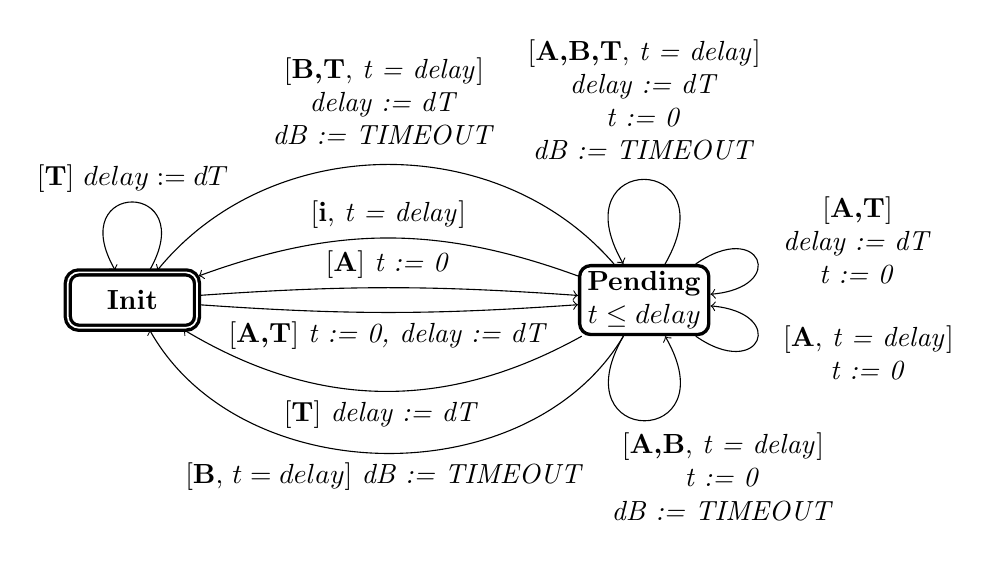
\begin{tikzpicture}
    % State: ACK with different content
    \node[state, double,   	% layout (defined above)
    text width=1.5cm, 	% max text width    
    anchor=center] (init) 	% posistion relative to the center of the 'box'
    {\textbf{Init}};
    
    \node[state,    	% layout (defined above)
    text width=1.5cm, 	% max text width
    right of=init,
    node distance=6.5cm,
    anchor=center] (pending) 	% posistion relative to the center of the 'box'
    {\textbf{Pending}\\$t\leq delay$};
    
    % draw the paths and and print some Text below/above the graph
    \path
        (init)      edge[in=176,out=4, ->] 
            node[above] {[\textbf{A}] \emph{t := 0}} 
        (pending)

        (init)      edge[->, in=184, out=-4] 
            node[below] {[\textbf{A,T}] \emph{t := 0, delay := dT}} 
        (pending)

        (init)      edge[loop, ->,in=120,out=60, looseness=8]
            node[above] {[\textbf{T}] $delay:=dT$}
        (init)

        (pending)   edge[bend left=60, ->]
            node[below] {[\textbf{B}, $t= delay$] \emph{dB := TIMEOUT}}
        (init)

        (pending)   edge[bend left, ->]
            node[below] {[\textbf{T}] \emph{delay := dT}}
        (init)

        (pending)   edge[bend right=20, ->]
            node[above] {[\textbf{i}, \emph{t = delay}]}
        (init)

        (pending)      edge[loop, ->,in=120,out=60, looseness=8]
            node[above] {
                \begin{tabular}{c}
                    [\textbf{A,B,T}, \emph{t = delay}] \\
                    \emph{delay := dT} \\
                    \emph{t := 0} \\
                    \emph{dB := TIMEOUT}
                \end{tabular}
            }
        (pending)

        (pending)      edge[loop, ->,in=5,out=35, looseness=6]
            node[right, yshift=0.2cm] {
                \begin{tabular}{c}
                    [\textbf{A,T}] \\
                    \emph{delay := dT} \\
                    \emph{t := 0}
                \end{tabular}
            }
        (pending)

        (pending)      edge[loop, ->,in=-5,out=-35, looseness=6]
            node[right, yshift=-0.2cm] {
                \begin{tabular}{c}
                    [\textbf{A}, \emph{t = delay}] \\
                    \emph{t := 0}
                \end{tabular}
            }
        (pending)

        (pending)      edge[->, bend right=50]
            node[above] {
                \begin{tabular}{c}
                    [\textbf{B,T}, \emph{t = delay}] \\
                    \emph{delay := dT} \\
                    \emph{dB := TIMEOUT}
                \end{tabular}
            }
        (init)

        (pending) edge[loop,->,in=-60,out=-120, looseness=8]
            node [below, xshift=1cm] {
                \begin{tabular}{c}
                    [\textbf{A,B}, \emph{t = delay}] \\
                    \emph{t := 0} \\
                    \emph{dB := TIMEOUT}
                \end{tabular}
            }
        (pending)
        ;
        
\end{tikzpicture}
            }
            \caption{Semantics of pTimer}
            \label{fig:pTimer}
        \end{figure}
\end{description}

\subsection{Composition of Connectors as $\nSTA$}

As mentioned before, connectors in Reo are constructed from simpler ones in a compositional approach. Now we show how connectors are composed by \emph{product} and \emph{hiding} operations on $\nSTA$.

% The formal definition of $\nSTA$ has been specified hereinbefore. In this section, we will provide the compositional semantics for Reo connectors. As the replicate and merge operations have been specified as channels, we have no need to consider mixed nodes with multiple inputs or multiple outputs. On the automata level, the join of a flow-through node that we only need to consider will be implemented by the $product$ construction. Specifically, $product$ and $hiding$ operators are defined for $\nSTA$ to obtain the semantics of a stochastic timed Reo connector out of the $\nSTA$ corresponding to its basic channels.

The \emph{product} operator is used to combine two connectors by joining their \emph{shared nodes} (\emph{shared actions} in $\nSTA$). In \emph{product} operations, we always assume that shared actions have the same identifiers, while other variables and clocks are all named without repetition. Before showing the formal definition of the \emph{product} operator, first we introduce a predicate \emph{compatible}.

\begin{definition}[Compatible $\nSTA$]
    Let $\mathscr{A}_{i}=\langle L_{i}, l_{0,i}, Acts_{i}, V_{i}, V_{0,i}, C_{i}, Inv_{i}, E_{i} \rangle$ be two $\nSTA$ (i=1,2), they are compatible if
    \begin{itemize}
        \item there's no conflicting initialization on shared variables, formalized as $\forall v\in V_1\cap V_2, V_{0,1}(v) = V_{0,2}(v)$, and
        \item shared variables can only be assigned in one of them, i.e. if $v\in V_1\cap V_2$ and $v:=expr$ ($expr$ is an expression) appears in the assignments of $\mathscr{A}_1$, then $\forall e\in E_2$, e should not contain any assignment on $v$, and vice versa.
    \end{itemize}
    In other words, we don't allow two connectors to write on the same node. 
\end{definition}

\begin{definition}[Product]
Let $\mathscr{A}_{i}=\langle L_{i}, l_{0,i}, Acts_{i}, V_{i}, V_{0,i}, C_{i}, Inv_{i}, E_{i} \rangle(i=1,2)$ be two compatible $\nSTA$, their product $\mathscr{A}=\mathscr{A}_{1}\bowtie \mathscr{A}_{2}$ is defined as:
\[
    \mathscr{A}_{1}\bowtie \mathscr{A}_{2}=\langle L_1\times L_2, (l_{0,1}, l_{0,2}), Acts_1\cup Acts_2, V_{1}\cup V_{2}, V_0, C_{1}\cup C_{2}, Inv, E\rangle
\]
where
\begin{itemize}
    \item $V_0(v)$ is equal to $V_{0,1}(v)$ if $v\in V_1\backslash V_2$, or $V_{0,2}(v)$ otherwise,
    \item $Inv(l_1,l_2)(ev)=Inv_1(l_1)(\restrict{ev}{V_1\cup C_1})\land Inv_2(l_2)(\restrict{ev}{V_2\cup C_2})$, where $\restriction$ is used to restrict a function on certain domain,
    \item $E$ is obtained through the following rules:
        \begin{equation}
            \frac{l_{1}\xrightarrow{\textbf{acts}_{1},g_{1},u_{1}}_{E_1} l_{1}', acts_{1}\cap Acts_{2}=\varnothing}{\langle l_{1},l_{2}\rangle\xrightarrow{\textbf{acts}_{1},g_{1},u_{1}}_E\langle l_{1}',l_{2}\rangle}
        \end{equation}
        \begin{equation}
            \frac{l_{2}\xrightarrow{\textbf{acts}_{2},g_{2},u_{2}}_{E_2} l_{2}', acts_{2}\cap Acts_{1}=\varnothing}{\langle l_{1},l_{2}\rangle\xrightarrow{\textbf{acts}_{2},g_{2},u_{2}}_E\langle l_{1},l_{2}'\rangle}
        \end{equation}
        \begin{equation}
            \label{equ:product}
            \frac{l_{1}\xrightarrow{\textbf{acts}_{1},g_{1},u_{1}}_{E_1} l_{1}', l_{2}\xrightarrow{\textbf{acts}_{2},g_{2},u_{2}}_{E_2} l_{2}',acts_{1}\cap Acts_{2}=acts_{2}\cap Acts_{1}}
        {\langle l_{1},l_{2}\rangle\xrightarrow{\textbf{acts}_{1}\cup \textbf{acts}_{2},g, u}_E\langle l_{1}',l_{2}'\rangle}
        \end{equation}
\end{itemize}
\end{definition}
% \item{$V_0$ is an initialized function obtained by assigning values to variables in $\mathscr{A}_{1}$ according to the initialization $V_{0,1}$ and assigning values to variables in $\mathscr{A}_{2}$ according to the initialization $V_{0,2}$.}
% \item{A finite set of actions $Acts = Acts_{1}\cup Acts_{2}$.}
% \item{$Inv$ is a function that assigns an invariant to each location which is obtained by $Inv(l_{1}, l_{2}) = Inv_{1}(l_{1})\wedge Inv_{2}(l_{2})$.}
% \item{A finite set of edges $E$ is obtained through the rules which are shown in Definition 4.}
% \end{itemize}

In rule~(\ref{equ:product}), guard formula is the logical conjunction of $g_1$ and $g_2$, formally $g(ev)=g_1(\restrict{ev}{V_1\cup C_1})\land g_2(\restrict{ev}{V_2\cup C_2})$ is defined simply following \emph{Inv}. However, the definition of $u$ is much more complicated. For example, in Fig.~\ref{fig:prodsyncandfifo} we may have \emph{dB := dA} as $u_1$, and \emph{dC := dB} as $u_2$. Their direct product is \emph{dB := dA, dC := dB}. Obviously, we need an order here to resolve the dependency between variables (otherwise these statements could become a great mess), which is provided as follows.

\begin{enumerate}
    \item Check all the assignment statements $v:=expr$ in $u_1$, and use expression $expr$ to replace all the existence of $v$ in both $u_2$ and $g_2$,
    \item Reversely, check all $v:=expr$ in $u_2$, and replace their existence in both $u_1$ and $g_1$ (note that this replacement will also affect $g$),
    \item Repeat the previous steps until nothing can be replaced,
    \item Suppose $u_1'$ and $u_2'$ are the resolved assignment statements, we have
        \begin{displaymath}
            u(v)=\left\{
            \begin{array}{lr}
                u_1'(v) & \hspace{1cm}\mbox{$v$ is assigned in $v_1$}, \\
                u_2'(v) & otherwise
            \end{array}
            \right.
        \end{displaymath}
\end{enumerate}

%Correctness of these steps highly relies on the \emph{compatible} assumption \xy{which ensures} that we don't need to resolve assignment statements like \emph{a := b, b := a}.

With the $product$ operator, we can obtain a rough combination of Reo connectors (as $\nSTA$). But there are still redundant statements that should have been simplified. We now introduce the $hiding$ operator which can be used to omit such unnecessary parts.

\begin{definition}[Hideable Action]
    Let $\mathscr{A}= \langle L, l_0, Acts, V, V_0, C, Inv, E\rangle$ be a $\nSTA$ and $A\in Acts$ is an action. We say $A$ is hideable in $\mathscr{A}$ if a) all the assignment statements do not depend on the value of $dA$ (i.e. $dA$ never appears on the right-hand side of any assignment statement), and b) $dA$ doesn't appear in any guard or invariant.
\end{definition}

\begin{definition}[Hiding]
Let $\mathscr{A}= \langle L, l_0, Acts, V, V_0, C, Inv, E\rangle$ be a $\nSTA$ and $A\in Acts$ is a \emph{hideable} action in $\mathscr{A}$. The hiding operator $\mathscr{A}\backslash\{A\}$ is defined as
\begin{equation*}
\mathscr{A}\backslash\{A\}
=\langle L, l_0, V\backslash \{dA\}, \restrict{V_0}{V\backslash \{dA\}}, C, Acts\backslash\{A\}, Inv, E'\rangle
\end{equation*}
where $E'=\{\langle l, acts\backslash\{A\}, g, \restrict{u}{V\backslash \{dA\}}, l'\rangle | \langle l, acts, g, u, l'\rangle\in E\}$.
\end{definition}

Hiding operation can be also used to remove multiple hideable actions at a time. For example, we introduce the following notation, and it it easy to prove that this notation is well-defined, and satisfies the law of commutation (since all we do in hiding is to remove things from existing terms).
\[
    \mathscr{A}\backslash \{A_1,\cdots, A_n\}:=\mathscr{A}\backslash \{A_1\}\backslash\{A_2\}\cdots\backslash \{A_n\}
\]

% The well-defined definition of hiding operator depends on that we only have the flow-through operation to handle as the merge and replicate operations have been defined as channels. We also suppose that we always perform the merge and replicate operations first and perform the flow-through operation afterwards.
% Thus when taking the intersection of $V_{1}$ and $V_{2}$, we don't need to worry about whether $V_{h}$, i.e. the intersection, is obtained from replicate, merge or flow-through operations.

We consider a simple example in Fig.~\ref{fig:prodsyncandfifo}, where we use \emph{product} and \emph{hiding} operators to combine a \emph{Sync} and a \emph{FIFO1} channel. In Fig.~\ref{fig:prodsyncandfifo}, we show the combined connector in different stages and its corresponding $\nSTA$ step by step.

\begin{figure}[H]
    \centering
    \resizebox{.85\textwidth}{!}{
        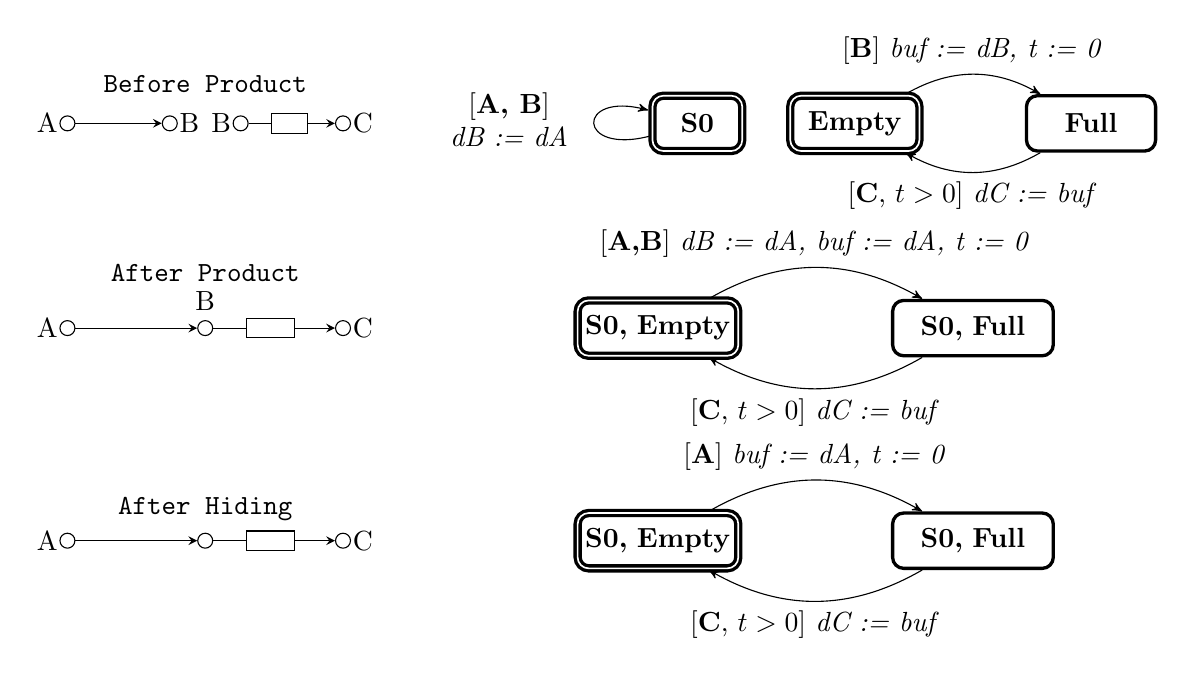
\begin{tikzpicture}[>=stealth']
    % draw the connector
    \node (bfp) at (-4.25, 3.1) {\tt Before Product};
    \node (bfp) at (-4.25, 0.7) {\tt After Product};
    \node (bfp) at (-4.25, -2.3) {\tt After Hiding};

    \ionode{(A)}{(-6, 2.6)}{node[left] {A}};
    \ionode{(B1)}{(-4.7, 2.6)}{node[right] {B}};
    \ionode{(B2)}{(-3.8, 2.6)}{node[left] {B}};
    \ionode{(C)}{(-2.5, 2.6)}{node[right] {C}};
    \sync{(A)}{(B1)}{}
    \fifoe{(B2)}{(C)}{}

    \ionode{(Ad)}{(-6, 0)}{node[left] {A}};
    \ionode{(Bd)}{(-4.25, 0)}{node[above=0.1cm] {B}};
    \ionode{(Cd)}{(-2.5, 0)}{node[right] {C}};
    \sync{(Ad)}{(Bd)}{}
    \fifoe{(Bd)}{(Cd)}{}

    \ionode{(Ah)}{(-6, -2.7)}{node[left] {A}};
    \ionode{(Bh)}{(-4.25, -2.7)}{};
    \ionode{(Ch)}{(-2.5, -2.7)}{node[right] {C}};
    \sync{(Ah)}{(Bh)}{}
    \fifoe{(Bh)}{(Ch)}{}

    % State: ACK with different content
    \node[state,  double,   	% layout (defined above)
    text width=1.9cm, 	% max text width
    anchor=center] (init) at (1.5,0)	% posistion relative to the center of the 'box'
    {\textbf{S0, Empty}};

    \node[state,    	% layout (defined above)
    text width=1.9cm, 	% max text width
    right of=init,
    node distance=4cm,
    anchor=center] (ready) 	% posistion relative to the center of the 'box'
    {\textbf{S0, Full}};

    % draw the paths and and print some Text below/above the graph
    \path
        (ready)   edge[bend left, ->]
            node[below] {[\textbf{C}, $t > 0$] \emph{dC := buf}}
        (init)

        (init)  edge[bend left, ->]
            node[above] {[\textbf{A,B}] \emph{dB := dA, buf := dA, t := 0}}
        (ready);

    \node[state, double,   	% layout (defined above)
    text width=1.9cm, 	% max text width
    anchor=center] (hinit) at (1.5,-2.7)	% posistion relative to the center of the 'box'
    {\textbf{S0, Empty}};

    \node[state,    	% layout (defined above)
    text width=1.9cm, 	% max text width
    right of=hinit,
    node distance=4cm,
    anchor=center] (hready) 	% posistion relative to the center of the 'box'
    {\textbf{S0, Full}};

    % draw the paths and and print some Text below/above the graph
    \path
        (hready)   edge[bend left, ->]
            node[below] {[\textbf{C}, $t > 0$] \emph{dC := buf}}
        (hinit)

        (hinit)  edge[bend left, ->]
            node[above] {[\textbf{A}] \emph{buf := dA, t := 0}}
        (hready);

    % sync
    \node[state, double,   	% layout (defined above)
    text width=1cm, 	% max text width    
    anchor=center] (S0) 	% posistion relative to the center of the 'box'
    at (2, 2.6)
    {\textbf{S0}};

    \path (S0)  edge[loop left] node{
        \begin{tabular}{c}
            [\textbf{A, B}] \\
            \emph{dB := dA}
        \end{tabular}
    } (S0);

    % FIFO1
    \node[state,    	% layout (defined above)
    text width=1.5cm, 	% max text width
    node distance=3.6cm,
    anchor=center] (fifoready) 	% posistion relative to the center of the 'box'
    at (7,2.6)
    {\textbf{Full}};

    \node[state, double,   	% layout (defined above)
    text width=1.5cm, 	% max text width    
    left of=fifoready,
    node distance=3cm,
    anchor=center] (fifoinit) 	% posistion relative to the center of the 'box'
    {\textbf{Empty}};

    % draw the paths and and print some Text below/above the graph
    \path
        (fifoready)   edge[bend left, ->]
            node[below] {[\textbf{C}, $t > 0$] \emph{dC := buf}} 
        (fifoinit)

        (fifoinit)  edge[bend left, ->]
            node[above] {[\textbf{B}] \emph{buf := dB, t := 0}} 
        (fifoready);
\end{tikzpicture}

    }
    \caption{\emph{Product} and \emph{Hiding} of \emph{Sync(A,B)} and \emph{FIFO1(B,C)}}
    \label{fig:prodsyncandfifo}
\end{figure}

% Next we consider two Reo connectors both consisting of a $StochasticChoice$ channel and a $FIFO1$ channel but produced in a different order. As $StochasticChoice$ channel is a synchronous channel, here we omit the $Ready$ state and the internal action. The two connectors are shown in Fig.~\ref{fig:compsyncfifo}.
% \begin{figure}
%     \centering
%     \begin{tikzpicture}
%         \ionode{(io1)}{(0.5,0)}{node[below]{A1}}
%         \ionode{(io2)}{(4.5,0)}{node[below]{C1}}
%         \ionode{(io3)}{(6.5,0)}{node[below]{A2}}
%         \ionode{(io4)}{(10.5,0)}{node[below]{C2}}
%         \mixednode{(m1)}{(2.5,0)}{node[below]{B1}}
%         \mixednode{(m2)}{(8.5,0)}{node[below]{B2}}
%         \sync{(io1)}{(m1)}{node[below]{$dist$}}
%         \fifoe{(m1)}{(io2)}{}
%         \fifoe{(io3)}{(m2)}{}
%         \sync{(m2)}{(io4)}{node[below]{$dist$}}
%     \end{tikzpicture}
%     \caption{Composition of StochasticChoice and FIFO1 channel.}
%     \label{fig:compsyncfifo}
% \end{figure}

% \begin{comment}
% The products of $\nSTA$ corresponding to these two connectors with different composition orders are shown in Fig.~\ref{fig:prostofifo}.
% \begin{figure}[htbp]
% \centering
% \subfigure[1]{
% \begin{minipage}{5.5cm}
% \centering
% 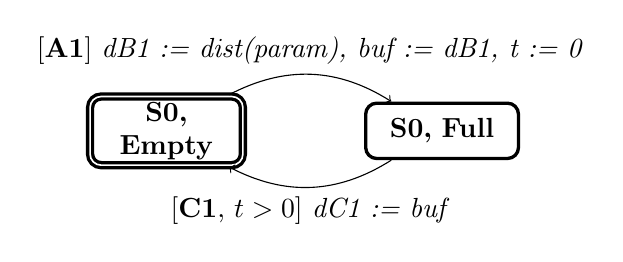
\begin{tikzpicture}
    % State: ACK with different content
    \node[state, double,   	% layout (defined above)
    text width=1.8cm, 	% max text width
    anchor=center] (init) 	% posistion relative to the center of the 'box'
    {\textbf{S0, Empty}};

    \node[state,    	% layout (defined above)
    text width=1.8cm, 	% max text width
    right of=init,
    node distance=3.5cm,
    anchor=center] (ready) 	% posistion relative to the center of the 'box'
    {\textbf{S0, Full}};

    % draw the paths and and print some Text below/above the graph
    \path
        (ready)   edge[bend left, ->]
            node[below] {[\textbf{C1}, $t > 0$] \emph{dC1 := buf}}
        (init)

        (init)  edge[bend left, ->]
            node[above] {[\textbf{A1}] \emph{dB1 := dist(param), buf := dB1, t := 0}}
        (ready);
\end{tikzpicture}

% \end{minipage}
% }
% %\label{fig:syncchoiceandfifo}
% \subfigure[2]{
% \begin{minipage}{5.5cm}
% \centering
% 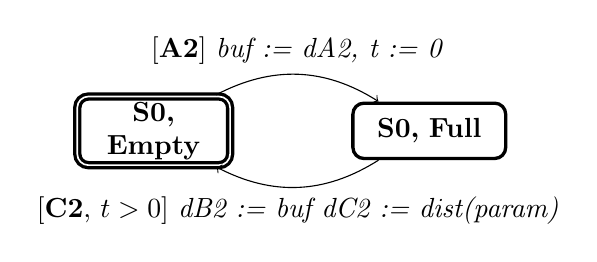
\begin{tikzpicture}
    % State: ACK with different content
    \node[state,  double,   	% layout (defined above)
    text width=1.8cm, 	% max text width
    anchor=center] (init) 	% posistion relative to the center of the 'box'
    {\textbf{S0, Empty}};

    \node[state,    	% layout (defined above)
    text width=1.8cm, 	% max text width
    right of=init,
    node distance=3.5cm,
    anchor=center] (ready) 	% posistion relative to the center of the 'box'
    {\textbf{S0, Full}};

    % draw the paths and and print some Text below/above the graph
    \path
        (ready)   edge[bend left, ->]
            node[below] {[\textbf{C2}, $t > 0$] \emph{dB2 := buf dC2 :=  dist(param)}}
        (init)

        (init)  edge[bend left, ->]
            node[above] {[\textbf{A2}] \emph{buf := dA2, t := 0}}
        (ready);
\end{tikzpicture}

% \end{minipage}
% }
% \caption{Product of StochasticChoice and FIFO1}
% \label{fig:prostofifo}
% \end{figure}
% \end{comment}

% After performing the $product$ and $hiding$ operators, we can see the final result. Although the basic channels are the same, there are some differences between the two final products, which results from different locations where probabilistic behavior happens.
% In the first Reo connector, data items arriving in $B1\in StochasticChoice.Acts$ are stochastic. Following that, whatever the data item is, it is stored into the buffer of FIFO1 deterministically. Nevertheless, in the second Reo connector, no matter what the data item taken from the buffer is, the output of the connector will totally depend on the parameter $dist$ of $StochasticChoice$ channel.
% \begin{figure}[htbp]
% \centering
% \subfigure[1]{
% \begin{minipage}{5.5cm}
% \centering

% 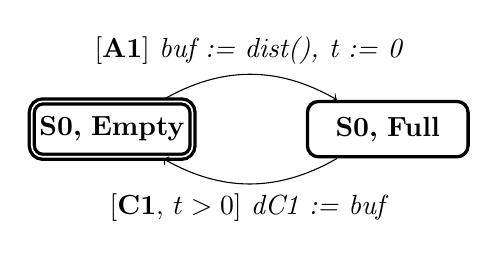
\begin{tikzpicture}
    % State: ACK with different content
    \node[state,  double,   	% layout (defined above)
    text width=1.9cm, 	% max text width
    anchor=center] (init) 	% posistion relative to the center of the 'box'
    {\textbf{S0, Empty}};

    \node[state,    	% layout (defined above)
    text width=1.9cm, 	% max text width
    right of=init,
    node distance=3.5cm,
    anchor=center] (ready) 	% posistion relative to the center of the 'box'
    {\textbf{S0, Full}};

    % draw the paths and and print some Text below/above the graph
    \path
        (ready)   edge[bend left, ->]
            node[below] {[\textbf{C1}, $t > 0$] \emph{dC1 := buf}}
        (init)

        (init)  edge[bend left, ->]
            node[above] {[\textbf{A1}] \emph{buf := dist(), t := 0}}
        (ready);
\end{tikzpicture}

% \end{minipage}
% }
% %\label{fig:syncchoiceandfifo}
% \subfigure[2]{
% \begin{minipage}{5.5cm}
% \centering
% 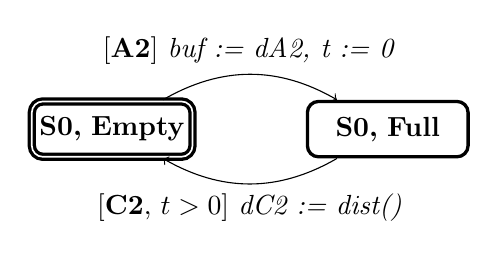
\begin{tikzpicture}
    % State: ACK with different content
    \node[state, double,    	% layout (defined above)
    text width=1.9cm, 	% max text width
    anchor=center] (init) 	% posistion relative to the center of the 'box'
    {\textbf{S0, Empty}};

    \node[state,    	% layout (defined above)
    text width=1.9cm, 	% max text width
    right of=init,
    node distance=3.5cm,
    anchor=center] (ready) 	% posistion relative to the center of the 'box'
    {\textbf{S0, Full}};

    % draw the paths and and print some Text below/above the graph
    \path
        (ready)   edge[bend left, ->]
            node[below] {[\textbf{C2}, $t > 0$] \emph{dC2 :=  dist()}}
        (init)

        (init)  edge[bend left, ->]
            node[above] {[\textbf{A2}] \emph{buf := dA2, t := 0}}
        (ready);
\end{tikzpicture}

% \end{minipage}
% }
% \caption{Final Product of StochasticChoice and FIFO1}
% \end{figure}

% \subsection{Commutative and Associative Law}
\subsection{Well-definedness of Composition Operators}

To specify the well-definedness of composition operators listed above, here we present the \emph{commutative} law and the \emph{associative} law for them. Before starting, first we introduce the \emph{isomorphism} of $\nSTA$.


\begin{definition}[Isomorphism]
    \label{def:isomorphism}
    Two $\nSTA$ are \emph{isomorphic} ($\mathscr{A}_1\cong\mathscr{A}_2$, where $\mathscr{A}_{i}=\langle L_{i}, l_{0,i}, Acts_{i}, V_{i}, V_{0,i}, C_{i}, Inv_{i}, E_{i}\rangle$), if the 1-to-1 mappings $f_L:L_1\rightarrow L_2$, $f_V:V_1\rightarrow V_2$, $f_C:C_1\rightarrow C_2$, $f_{act}:Acts_1\rightarrow Acts_2$
    exist and satisfy:
    \begin{itemize}
        \item $f_L(l_{0,1}) = l_{0,2}$, 
        \item $\forall v\in V_1, V_{0,1}(v) = V_{0,2}(f_V(v))$,
        \item $\forall l\in L_1, Inv_1(l)$ and $Inv_2(f_L(l))$ can be obtained from each other by variables' replacement specified by $f_V$ and $f_C$,
        \item $\forall e=\langle l, acts, g , u, l' \rangle \in E_1$, we can find a corresponding exclusive edge $e'\in E_2 = \langle f_L(l), \{f_{act}(a)|a\in acts\}, g', u', f_L(l')\rangle$
        where $g',u'$ and $g,u$ can be obtained from each other by variables' replacement specified by $f_V$ and $f_C$.
    \end{itemize}
\end{definition}

Informally speaking, two $\nSTA$ are isomorphic if they have the same graphical structure and homologous behavior, despite the slight difference of location labels or variable identifiers. The \emph{commutative} and \emph{associative} laws we present in the following are essentially based on the definition of \emph{isomorphism}.


% \ly{
%     Considering the graphical model of Reo, these laws are obvious and clear. For example, suppose there are three nodes $A$, $B$, $C$ and two connectors $conn_1(A,B)$, $conn_2(B,C)$. Joining $conn_2$ to $conn_1$ or $conn_1$ to $conn_2$, intuitively, will lead to exactly the same results. However, to illustrate this from a formal aspect of view, we still need to formalize and prove the law of communtation on its semantics $\nSTA$.
% }
% As for all nodes A, B, C, and channels, assume that one connector is the composition of two channels $chan1(A,B)$ and $chan2(B,C)$ and the other connector is the composition of $chan2(B,C)$ and $chan1(A,B)$, the result connectors are totally the same, which is a $chan1$ channel with source end $A$ and sink end $B$ immediately following a $chan2$ channel with source end $B$ and sink end $C$.
% For the other two composition operations merge and replicate, we specify them as channels. But we can also see the law of commutation is satisfied easily.


% However, the commutative law of $\nSTA$ corresponding to $channelname1$ and $channelname2$ is not so explicit as composition of channels.
\begin{theorem}[Commutative]
\label{thm:commutative}
Let $\mathscr{A}_1, \mathscr{A}_2$ be two $\nSTA$, $\mathscr{A}_{1}\bowtie \mathscr{A}_{2}\cong\mathscr{A}_{2}\bowtie \mathscr{A}_{1}$.
\end{theorem}

% Considering in a similar way, we can easily obtain the law of association for the composition of Reo connectors. For three channels, assume that the first one is $channelname1$ with source end $A$ and sink end $B$, the second one is $channelname2$ with source end $B$ and sink end $C$ and the last is $channelname3$ with source end $C$ and sink end $D$. We can combine the three channels in two different orders. However, in either order, we will always obtain a connector which is $channelname1$ followed by $channelname2$ followed by $channelname3$ with source end $A$, sink end $D$ and two hiding ends $B$,$C$.

% For the other two composition operations merge and replicate, we already specify them as channels. Nevertheless, for three channels, when composing them in either order, the result of replicate is that data items will be replicated into three channels and the result of merge is that data items will be taken from three channels nondeterministically. Thus, the two composition operations merge and replicate also satisfy the law of association.

% As for associative law of $\nSTA$ corresponding to three channels, it can be formulated as follows.
\begin{theorem}[Associative]
\label{thm:associative}
Let $\mathscr{A}_1, \mathscr{A}_2, \mathscr{A}_3$ be three $\nSTA$, ($\mathscr{A}_{1}\bowtie \mathscr{A}_{2})\bowtie \mathscr{A}_{3}\cong\mathscr{A}_{1}\bowtie(\mathscr{A}_{2}\bowtie \mathscr{A}_{3})$.
\end{theorem}


From the two theorems above, it's clear that orders make only little difference in composition of $\nSTA$. No matter how we label the identifiers and write the composing expression, finally the connectors we obtain have the same behavior. Similar to the isomorphism of graphs, these laws can be easily proved through a constructive approach.

    \section{Case Studies}
\label{sec:casestudies}


With support of the composition operators, Reo can be used to capture various coordination scenarios in the real world. In this section, we present two examples: \emph{Probabilistic Router} and \emph{Expiring Timer}.


\begin{example}[Probabilistic Router]
\emph{Router} is a widely used connector example \cite{Baier2006a,Arbab2006}. As shown in Fig.~\ref{fig:router} (a), a \emph{Router} uses two \emph{LossySync} channels and a \emph{SyncDrain} channel to make sure that a coming data value is only sent to one of its sink ends. This choice is made nondeterministically at $C$, where the \emph{Merger} channel exists. Here we show how the nondeterministic behavior is resolved as probabilistic behavior through the \emph{StochasticChoice} channel.


\begin{figure}[t]
    \centering
    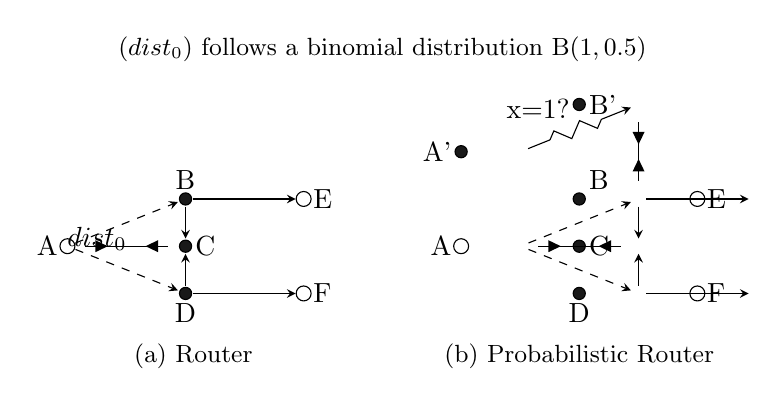
\begin{tikzpicture}
    % part 1. router
    \node (note) at (4,2.5) {\small
        ($dist_0$) follows a binomial distribution $\operatorname{B}(1,0.5)$
    };

    \node (note1) at (1.6, -1.4) {\small (a) Router};
    \node (note2) at (6.5, -1.4) {\small (b) Probabilistic Router};

    \ionode{(in)}{(0, 0)}{node[left] {A}}
    \ionode{(outup)}{(3, 0.6)}{node[right] {E}}
    \ionode{(outdown)}{(3, -0.6)}{node[right] {F}}
    \mixednode{(mid)}{(1.5, 0)}{node[right] {C}}
    \mixednode{(wayup)}{(1.5, 0.6)}{node[above] {B}}
    \mixednode{(waydown)}{(1.5, -0.6)}{node[below] {D}}

    \lossysync{(in)}{(wayup)}{}
    \lossysync{(in)}{(waydown)}{}
    \syncdrain{(in)}{(mid)}{}
    \sync{(wayup)}{(mid)}{}
    \sync{(waydown)}{(mid)}{}

    \sync{(wayup)}{(outup)}{}
    \sync{(waydown)}{(outdown)}{}

    \ionode{(pin)}{(5, 0)}{node[left] {A}}
    \ionode{(poutup)}{(8, 0.6)}{node[right] {E}}
    \ionode{(poutdown)}{(8, -0.6)}{node[right] {F}}
    \mixednode{(pmid)}{(6.5, 0)}{node[right] {C}}
    \mixednode{(pwayup)}{(6.5, 0.6)}{node[above right] {B}}
    \mixednode{(pmap1)}{(5, 1.2)}{node [left] {A'}}
    \mixednode{(pmap2)}{(6.5, 1.8)}{node [right] {B'}}
    \mixednode{(pwaydown)}{(6.5, -0.6)}{node[below] {D}}

    \choice{(pin)}{(pmap1)}{node [left] {$dist_0$}}
    \filter{(pmap1)}{(pmap2)}{node [above left] {x=1?}}
    \syncdrain{(pmap2)}{(pwayup)}{}

    \lossysync{(pin)}{(pwayup)}{}
    \lossysync{(pin)}{(pwaydown)}{}
    \syncdrain{(pin)}{(pmid)}{}
    \sync{(pwayup)}{(pmid)}{}
    \sync{(pwaydown)}{(pmid)}{}

    \sync{(pwayup)}{(poutup)}{}
    \sync{(pwaydown)}{(poutdown)}{}
\end{tikzpicture}

    \caption{From Router to Probabilistic Router}
    \label{fig:router}
\end{figure}

We attach a new path $A\rightarrow A'\rightarrow B'\rightarrow B$ to the original \emph{Router}, including a \emph{StochasticChoice}, a \emph{Filter} and a \emph{SyncDrain}, as depicted in Fig.~\ref{fig:router} (b).
When the \emph{StochasticChoice} channel is triggered, numeric value $0$ or $1$ will be generated, and in turn passed to the \emph{Filter} channel. If the value is $1$, it will be sent to the \emph{SyncDrain} channel $BB'$. In this case, the incoming value has to go through the path $A\rightarrow B\rightarrow E$. Otherwise, if the sampled value is $0$, it will be dropped by the \emph{Filter}, the incoming value will be sent to $F$ as $B$ cannot accept any data from $A$.

% which ensures that the outputs randomly choose two sink ends accordinging to the distrubution, i.e. with the same probability.
% Generally speaking, the random router keeps the same structure with its original version, i.e. one source end and two sink ends, but
% the probabilistic behavior is in consideration.
% To alter the probability of two ends receiving data items, only the parameter of the $StochasticChoice$ channel need update.
% In this way, the nondeterministic router can be turned into a probabilistic router with controllable probability and distribution. 

The corresponding $\nSTA$ of a \emph{Probabilistic Router} can be deduced on the basis of primitive channels' semantics and product operators.
There are two locations in the product $\nSTA$, since the primitive channels in the connector are all synchronous (including only one location) except the \emph{StochasticChoice} channel (having two locations). According to the \emph{product} operator, the locations should be labelled as tuples like \emph{(S0,...,Init,...)}. Here for simplicity we use \emph{Init} and \emph{Ready} instead.
The final result $\nSTA$, after \emph{hiding} all the internal nodes except \emph{A,E,F}, is shown in Fig.~\ref{fig:probabilistic_router}. 
\begin{figure}[H]
\centering
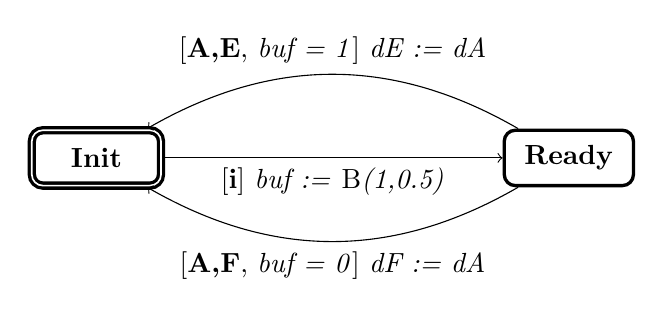
\begin{tikzpicture}
    % State: ACK with different content
    \node[state, double,   	% layout (defined above)
    text width=1.5cm, 	% max text width
    anchor=center] (init) 	% posistion relative to the center of the 'box'
    {\textbf{Init}};

    \node[state,    	% layout (defined above)
    text width=1.5cm, 	% max text width
    right of=init,
    node distance=6cm,
    anchor=center] (ready) 	% posistion relative to the center of the 'box'
    {\textbf{Ready}};

    % draw the paths and and print some Text below/above the graph
    \path
        (init)   edge[->]
            node[below] {[\textbf{i}] \emph{buf := }$\operatorname{B}$\emph{(1,0.5)}}
        (ready)

        (ready)  edge[bend left=30, ->]
            node[below] {[\textbf{A,F}, \emph{buf = 0}] \emph{dF := dA}}
        (init)

        (ready)  edge[bend right=30, ->]
            node[above] {[\textbf{A,E}, \emph{buf = 1}] \emph{dE := dA}}
        (init);
\end{tikzpicture}

\caption{$\nSTA$ of Probabilistic Router}
\label{fig:probabilistic_router}
\end{figure}
\end{example}

% \begin{example}[Embedded Control System]
% A common embedded control system usually comprises a set of sensors to obtain information from the environment, a set of actuators to operate on the environment, and a main processor to process information and give instructions. In the following we show how to use Reo connectors to formalize the coordination part of an embedded control system, which is a simplified version of the embedded controller model with modular redundancy in \cite{Kwia2007}.
% %\ly{
% %    \cite{Kwia2007} proposed an embedded controller model with modular redundancy.  In this paper, we simplify the original model (otherwise the connector would be too complicated to present), and show how to formalize its coordination part as a Reo connector under our framework.
% %}

% \begin{figure}[H]
%     \centering
%     \resizebox{.8\textwidth}{!}{
%         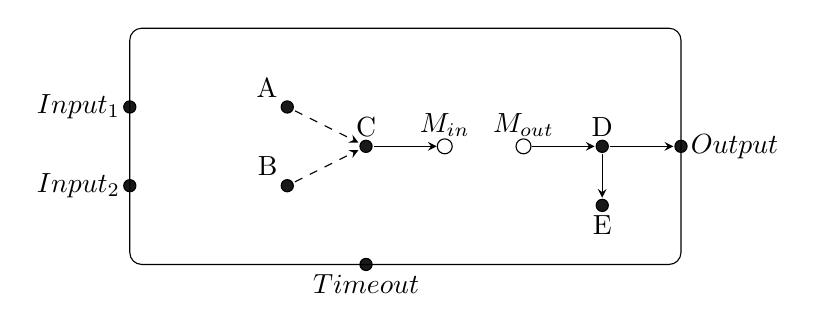
\begin{tikzpicture}
    \mixednode{(i1)}{(1, 1)}{node[left] {$Input_1$}}
    \mixednode{(i2)}{(1, 0)}{node[left] {$Input_2$}}

    \mixednode{(a)}{(3, 1)}{node[above left] {A}}
    \mixednode{(b)}{(3, 0)}{node[above left] {B}}

    \mixednode{(c)}{(4, 0.5)}{node[above ] {C}}
    \mixednode{(f)}{(4, -1.)}{node[below] {$Timeout$}}

    \mixednode{(d)}{(7, 00.5)}{node[above] {D}}
    \mixednode{(e)}{(7, -.25)}{node[below] {E}}

    \mixednode{(o)}{(8, 0.5)}{node[right] {$Output$}}

    \ionode{(m1)}{(5, 0.5)}{node[above] {$M_{in}$}}
    \ionode{(m2)}{(6, 0.5)}{node[above] {$M_{out}$}}

    \blackbox{(i1)}{(a)}{PF}{}
    \blackbox{(i2)}{(b)}{PF}{}

    \lossysync{(a)}{(c)}{}
    \lossysync{(b)}{(c)}{}

    \sync{(c)}{(m1)}{}
    \sync{(m2)}{(d)}{}

    \vrtimer{(c)}{(e)}{(f)}{RT}{}

    \sync{(d)}{(e)}{}
    \sync{(d)}{(o)}{}

    \component{(1,-1)}{(8,2)}{}

\end{tikzpicture}

%     }
%     \caption{Embedded Control System}
%     \label{fig:em}
% \end{figure}

% Sensors, actuators and the main processor are all regarded as components in this example.
% The assumption is, all the components are reliable but their communication is not. Such behavior is captured by a \emph{Probabilistic Filter} connector \textbf{PF} which is defined in Fig.~\ref{fig:em2}.
% The main processor, connected to ports \emph{$M_{in}$} and \emph{$M_{out}$},
% reads data coming from sensors, and passes instructions to the actuator
% through port \emph{Input} and \emph{Output}, respectively.
% The system fails to obtain an input only when both \emph{Probabilistic Filter}s fail.

% \begin{figure}[H]
%     \centering
%     \resizebox{.8\textwidth}{!}{
%         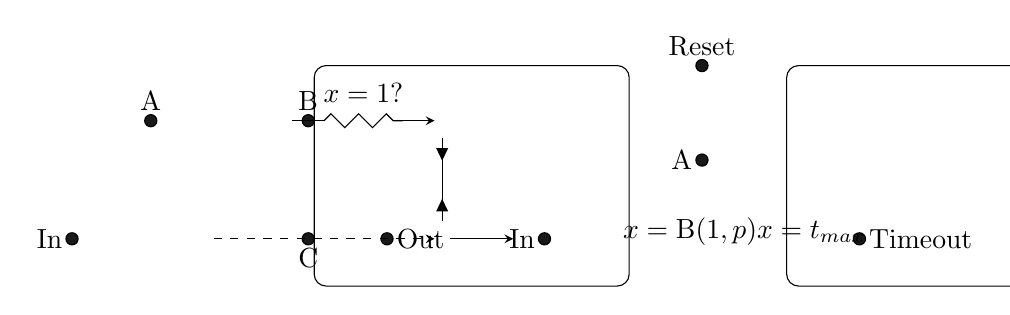
\begin{tikzpicture}
    %probabilistic filter
    \mixednode{(in1)}{(-7, 0)}{node[left] {In}}
    \mixednode{(a1)}{(-6, 1.5)}{node[above] {A}}
    \mixednode{(b1)}{(-4, 1.5)}{node[above] {B}}
    \mixednode{(c1)}{(-4, 0)}{node[below] {C}}
    \mixednode{(out1)}{(-3, 0)}{node[right] {Out}}

    %reset timer
    \mixednode{(in2)}{(-1, 0)}{node[left] {In}}
    \mixednode{(a2)}{(1, 1)}{node[left] {A}}
    \mixednode{(r2)}{(1, 2.2)}{node[above] {Reset}}
    \mixednode{(out2)}{(3, 0)}{node[right] {Timeout}}

    \choice{(in1)}{(a1)}{node [below right] {$x=\mathrm B(1, p)$}}
    \lossysync{(in1)}{(c1)}{}
    \sync{(c1)}{(out1)}{}
    \syncdrain{(b1)}{(c1)}{}
    \filter{(a1)}{(b1)}{node [above=3] {$x=1?$}}

    \choice{(r2)}{(a2)}{node [above right, xshift=0.1cm] {$x=t_{max}$}}
    \ptimer{(in2)}{(a2)}{(out2)}{}

    \component{(-7, -0.6)}{(-3, 2.2)}{}
    \component{(-1, -0.6)}{(3, 2.2)}{}

\end{tikzpicture}

%     }
%     \caption{Probablistic Filter (left) and Reset Timer (right)}
%     \label{fig:em2}
% \end{figure}

% In general, the main processor waits for potential input. However, due to the unreliable channels, we have to set a timeout mechanism to report system failures. In this model, a complete cycle (including data acquisition, data processing and instruction transmission) should be finished within a certain duration. Otherwise a \emph{timeout} signal will be generated by a \emph{Reset Timer} connector \textbf{RT}.

% A \emph{Probabilistic Filter} drops data with a certain probability, i.e. $1 - p$ in this example; while
% the \emph{Reset Timer} with time bound $t_{max}$ is a timer that supports reset operation (triggered by an extra source end \emph{Reset}). Reseting a \emph{Reset Timer} will prevent it from generating \emph{timeout} signals until it receives new value. The formal definition of \emph{Probabilistic Filter} and \emph{Reset Timer} is provided in Fig. \ref{fig:em2}. This also shows how Reo connectors are encapsulated and reused.

% There are 8 locations in the $\nSTA$ of the embedded system,
% consisting of triples which symbolizes the configuration of
%     two probabilistic filters and the reset timer.
% The corresponding $\nSTA$ represented in JANI format\cite{JaniSpec} is provided in Appendix.
% % elements are ommited except locations and edges.
% \end{example}

% \begin{example}[Delayed Channel]
% In this example, we propose an extension of delayed FIFO channels. It is obtained by replacing the timer channel with $StochasticTimer$ channel. The $SyncDrain$ channel serves to assure that the data item written at the source end can be taken exactly after a period of time randomly set by the $StochasticTimer$ channel. However, we can change the parameter of $StochasticTimer$ channel to meet some requirements. For example, if we want to delay the output by one time unit with greater probability or two units, we can set the $dist$ with $0.9\mapsto 1$ and $0.1\mapsto 2$. To a certain extent, it also reflects that a longer time delay interval is unbearable.
% \begin{figure}[H]
%     \centering
%     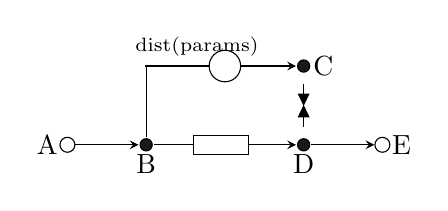
\begin{tikzpicture}
    % part 1. router
    \ionode{(in)}{(0, 0)}{node[left] {A}} 
    \mixednode{(wp1)}{(1, 0)}{node[below] {B}}
    \mixednode{(wp2)}{(3, 0)}{node[below] {D}}
    \mixednode{(wpup)}{(3, 1)}{node[right] {C}}
    \ionode{(out)}{(4, 0)}{node[right] {E}}

    \sync{(in)}{(wp1)}{}
    \fifoe{(wp1)}{(wp2)}{}
    \Lchannel{timer}{(wp1)}{(wpup)}{1}{v}{+}{node[above left] {\scriptsize dist(params)}}
    \syncdrain{(wpup)}{(wp2)}{}
    \sync{(wp2)}{(out)}{}
    

\end{tikzpicture}
%     \caption{Delayed Channel without Timeout}
% \end{figure}
% Urgency has to be considered in the aforementioned semantics, otherwise an inappropriate case will arise. The data item may be kept in the buffer and the timeout signal is just dropped in the meanwhile. If we don't consider urgency, the semantics which is exactly in the form of $\nSTA$ can be simply drawn as the following figure.

% \begin{figure}[H]
%     \centering
%     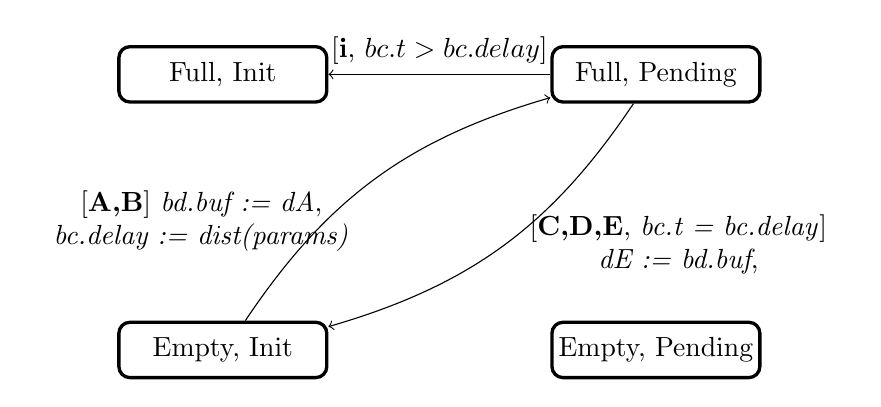
\begin{tikzpicture}
    % State: ACK with different content
    \node[state,    	% layout (defined above)
    text width=2.5cm, 	% max text width    
    anchor=center] (emptyinit) 	% posistion relative to the center of the 'box'
    {Empty, Init};
    
    \node[state,    	% layout (defined above)
    text width=2.5cm, 	% max text width
    right of=emptyinit,
    node distance=5.5cm,
    anchor=center] (emptypending) 	% posistion relative to the center of the 'box'
    {Empty, Pending};

    \node[state,    	% layout (defined above)
    text width=2.5cm, 	% max text width
    above of=emptyinit,
    node distance=3.5cm,
    anchor=center] (fullinit) 	% posistion relative to the center of the 'box'
    {Full, Init};

    \node[state,    	% layout (defined above)
    text width=2.5cm, 	% max text width
    right of=fullinit,
    node distance=5.5cm,
    anchor=center] (fullpending) 	% posistion relative to the center of the 'box'
    {Full, Pending};
    
    % draw the paths and and print some Text below/above the graph
    \path
        (emptyinit)   edge[bend left=20, ->] 
            node[below left] {
                \begin{tabular}{c}
                    [\textbf{A,B}] \emph{bd.buf := dA}, \\
                    \emph{bc.delay := dist(params)}
                \end{tabular}
            }
        (fullpending)

        (fullpending)   edge[bend left=20, ->] 
            node[right] {
                \begin{tabular}{c}
                    [\textbf{C,D,E}, \emph{bc.t = bc.delay}] \\
                    \emph{dE := bd.buf},
                \end{tabular}
            }
        (emptyinit)

        (fullpending) edge[->]
            node[above] {[\textbf{i}, $bc.t > bc.delay$]}
        (fullinit)
        ;
\end{tikzpicture}
%     \caption{Semantics of Delayed Channel without Timeout}
% \end{figure}
% \end{example}

\begin{example}[Expiring Timer]
    \label{exp:exptimer}
    
    In Timed Reo \cite{Meng2012}, different types of timer channels are proposed to capture real-time behaviors in different practical scenarios, including: \emph{OffTimer} that allows the timer to terminate the counting process when a certain signal is received, \emph{RSTTimer} that allows the timer to reset and restart its counting process, and \emph{EXPTimer} that makes the timer produce the TIMEOUT signal immediately when a certain signal is received.

    
    In this paper we take \emph{EXPTimer} as an example to show how \emph{pTimer} is used to encode the previous timers. In this example, the default delay time is denoted by $t$. (See Fig.~\ref{fig:exptimer})
    \begin{figure}
        \centering
        \resizebox{0.6\textwidth}{!}{
            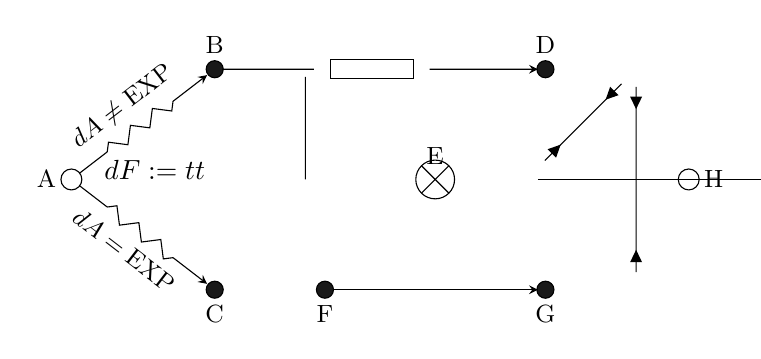
\begin{tikzpicture}[scale=1.4]

\tikzstyle{every node}=[font=\small]
\tikzstyle{label}=[draw=none]

\ionode{(A)}{(-0.3, 0)}{node [left=2] {A}}
\mixednode{(B)}{(1,1)}{node [above=2] {B}}
\mixednode{(C)}{(1,-1)}{node [below=2] {C}}
\mixednode{(D)}{(4,1)}{node [above=2] {D}}
\xrouter{(E)}{(3,0)}{node [above=2] {E}}
\mixednode{(F)}{(2,-1)}{node [below=2] {F}}
\mixednode{(G)}{(4,-1)}{node [below=2] {G}}
\ionode{(H)}{(5.3, 0)}{node [right=2] {H}}

\filter{(A)}{(B)}{node [xshift=-2,yshift=2,sloped,anchor=south,auto=false] {\small{$dA\neq \mbox{EXP}$}}}
\filter{(A)}{(C)}{node [xshift=-2,yshift=-2,sloped,anchor=north,auto=false] {\small{$dA=\mbox{EXP}$}}}
\fifoe{(B)}{(D)}{}
\sync{(F)}{(G)}{}
\map{(C)}{(F)}{node [above=2] {$dF:=t$}}
\map{(G)}{(H)}{node [xshift=-2,yshift=-2,sloped,anchor=north,auto=false] {\scriptsize{\emph{dH:=TIMEOUT}}}}
\sync{(E)}{(H)}{}

\syncdrain{(D)}{(E)}{}
\syncdrain{(D)}{(G)}{}

\draw (B) -- (1,0);
\ptimer{(1,0)}{(F)}{(E)}{node [above] {$t$}}

\end{tikzpicture}
        }
        \caption{Encode \emph{EXPTimer} with \emph{pTimer}}
        \label{fig:exptimer}
    \end{figure}
    
    Basically, this connector divide the incoming values into two classes: expiring signals and normal values. For a normal value, it goes into the \emph{pTimer} channel, and its copy is temporarily stored in the \emph{FIFO1} channel to show that the \emph{pTimer} is activated. When the counting process finished successfully without interruption, the buffered value will be dropped due to the \emph{SyncDrain} channel, and a TIMEOUT signal will be sent to $H$.

    On the other hand, when an expiring signal is caught, it will be replaced by the default delay value $t$ and sent to the $T$ end of the \emph{pTimer}. According to the semantics, the \emph{pTimer} will be reset immediately, and the buffered value will be dropped while sending out the TIMEOUT signal.
    
\end{example}

    \section{Discussion}
\label{sec:discussion}

In the coordination world, Reo is well known for its variety on extensions and semantics\cite{Jongmans2012}. And this is, of course, not the first work on its timed or stochastic semantics. Here we take \emph{timed Reo}, \emph{probabilistic Reo}, and \emph{stochastic Reo} as examples, to illustrate how our new model differs from its predecessors.

\vspace{0.5em}
\noindent{\emph{Timed Reo.}} Time was natively involved in Reo from its very beginning\cite{ARBAB2004}, where \emph{FIFO1} channel needs time constraints to ensure its retardancy. However, time was involved, only implicitly, in this semantics instead of syntax. And in some other semantics like \emph{constraint automata}, time is even simplified to logic order. Then \cite{Arbab2006} proposed the raw \emph{t-Timer} channels to capture timed delays. This work was then followed and extended in \cite{Meng2007} and \cite{Meng2012} with different types of timed channels.

The \emph{pTimer} channel here in our work is basically an improvement of t\emph{Timer} in \cite{Meng2012}. A \emph{Timer}t channel accepts data values and proceed timeout signals after a certain delay. However, it does not describe what happens if the timeout signal fails to deliver. In some cases, this will lead to timelock.

\emph{Timelock} have different meaning in different semantics. Informally speaking, a timed model falls into timelock if and only if there's no possible evolution that satisfies the model constraints, and hence the model execution is forced to stop. From a practical view, a connector suffering from timelock can not be simulated or implemented. And even in theoretical senarios \cite{Li2015}, it may also lead to inconsistency in proving frameworks as an unsatisfiable proposition \emph{False} derives everything.


\begin{example}[Timelock in Timed Reo]
    The \emph{Timer}t channels may easily lead to timelock. For example, in Fig.~\ref{fig:timelock}, there are two \emph{Timert}s, one is located between $A$ and $C$, the other between $B$ and $D$. According to the original definition of \emph{Timer}t in \cite{Arbab2006} and \cite{Meng2012}, we can derive that,
    \[
        \forall i\in\mathbb{N}, t_i(C)=t_i(A)+0.5, t_i(D)=t_i(B)+1,t_i(A)=t_i(B), t_i(C)=t_i(D)\quad (*)
    \]
    where $t(X)$ indicates the time stream on node $X$. For example, if $A$ accepts the first value at $0$, and the second value at $1$, then $t_0(A)=0,t_1(A)=1,\cdots$. From equation(*), it's easy to derive that $t(A) = t(A) + 0.5$. This connector will be trapped in timelock once $A$ starts accepting values.
    \begin{figure}[H]
        \centering
        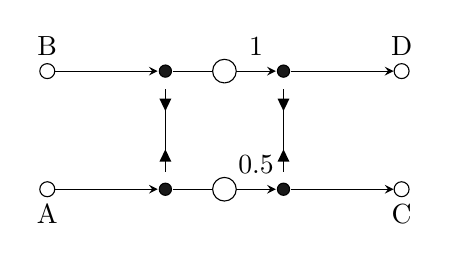
\begin{tikzpicture}
    \ionode{(A)}{(0,0)}{node [below=2] {A}}
    \ionode{(B)}{(0,1.5)}{node [above=2] {B}}
    \ionode{(C)}{(4.5,0)}{node [below=2] {C}}
    \ionode{(D)}{(4.5,1.5)}{node [above=2] {D}}

    \mixednode{(A1)}{(1.5,0)}{}
    \mixednode{(B1)}{(1.5,1.5)}{}
    \mixednode{(A2)}{(3,0)}{}
    \mixednode{(B2)}{(3,1.5)}{}

    \sync{(A)}{(A1)}{}
    \sync{(B)}{(B1)}{}
    \sync{(A2)}{(C)}{}
    \sync{(B2)}{(D)}{}

    \syncdrain{(A1)}{(B1)}{}
    \timer{(A1)}{(A2)}{node [above=2] {0.5}}
    \timer{(B1)}{(B2)}{node [above=2] {1}}
    \syncdrain{(A2)}{(B2)}{}

    % \ionode{(offIN)}{(5.5,0)}{}
    % \mixednode{(offA)}{(7,0)}{}
    % \xrouter{(offB)}{(8.5,0)}{}
    % \xrouter{(offC)}{(7, 1.5)}{}
    % \mixednode{(offD)}{(8.5,1.5)}{}
    % \mixednode{(offE)}{(10, 0)}{}
    % \mixednode{(offF)}{(10, 1.5)}{}
    % \mixednode{(offOUT)}{(11.5, .75)}{}

    % \sync{(offIN)}{(offA)}{}
    % \timer{(offA)}{(offB)}{node [above] {t}}
    % \syncdrain{(offC)}{(offD)}{}
    % \fifoe{(offA)}{(offC)}{}
    % \lossysync{(offB)}{(offE)}{}
    % \syncdrain{(offC)}{(offE)}{}
    % \fifoe{(offB)}{(offD)}{}
    % \sync{(offD)}{(offF)}{}
    % \sync{(offF)}{(offOUT)}{}
    % \sync{(offE)}{(offOUT)}{}
\end{tikzpicture}
        \label{fig:timelock}
        \caption{Timelock Caused by Abuse of \emph{Timer}t}
    \end{figure}
\end{example}

In comparison, \emph{pTimer} channels are timelock-free. If its sink end is not ready, the timeout signal will be dropped, and it channel will become available to accept new values again.

Further more, \emph{pTimer} channels also support reconfiguration of delay. In an original \emph{Timer}t channel, the delay is assigned when encoding the connector, and cannot be rewritten during execution. As a result, when formalizing specific timed connectors, we still need other channels like \emph{reset-timer}, \emph{expired-timer} and so on. In our framework, \emph{pTimer} is capable to represent all these channels with only simple combination patterns.

\vspace{0.5em}
\noindent{\emph{Probabilistic Reo.}} \cite{Models2005} came up with a probabilistic extension of constraint automata, to formalize the potential lossy behavior in connectors.

In \cite{Models2005}, probabilistic loss may happens while being transmitted or waiting in buffer. Definition of the former case is rather trivial, but in the latter one, discrete time is required and formalized as time units. The authors assume that in each time unit, a buffer failure may happens with probability $\tau$, and data values will get lost due to this failure.

In Section \ref{sec:casestudies}, we have already shown that probabilistic lossy channels can be represented by combination of \emph{StochasticChoice} channels and \emph{SyncDrain} channels. Actually, \emph{pTimer} channels is also capable to produce discrete time signals. Thus, we can use probablistic lossy channels and discrete time counters to reproduce the \emph{LossyFIFO1} in \cite{Models2005}.


\vspace{0.5em}
\noindent{\emph{Stochastic Reo.}} Baier and Wolf proposed the first stochastic extension for Reo in \cite{Baier2006} based on continuous-time constraint automata (CCA). The work was later extended with different semantics. For example, quantitative constraint automata in \cite{Arbab2009} and interactive markov chain in \cite{Oliveira2016}.

Basically, most of those stochastic semantics are based on continuous-time markov chains. Delays and arrival rates are attached to all the primitive channels, giving them randomized and unreliable behavior. This approach has a defect that random behavior is bounded with time. We can produce random delays but not random values. That's the reason why we split off stochastic delays as \emph{StochasticChoice}. \emph{StochasticChoice} has nothing to do with time, but we can always combine it with \emph{pTimer} to produce different timed connectors.


% \begin{figure}[H]
%     \centering
%     \begin{tikzpicture}
%         \ionode{(A)}{(0, 1.5)}{node [left=2] {A}}
%         \ionode{(Off)}{(0, 0)}{node [left=2] {Off}}

%         \mixednode{(A1)}{(1.5, 1.5)}{}
%         \mixednode{(B)}{(3, 1.5)}{}

%         \sync{(A)}{(A1)}{}
%         \timer{(A1)}{(B)}{}
%         \Uchannel{sync}{(0, 1.4)}{(2.25,1.4)}{0.4}{v}{-}{node [below=2] {$\{1\mapsto t\}$}}
%         \Lchannel{sync}{(Off)}{(2.25,1.4)}{2.25}{h}{+}{node [below=18] {$\{1\mapsto 0\}$}}
%     \end{tikzpicture}
% \end{figure}

% \begin{figure}[H]
%     \centering
%     \begin{tikzpicture}
%         \ionode{(IN)}{(-1.5,0)}{}
%         \ionode{(A)}{(0,0)}{}
%         \ionode{(B)}{(2,0)}{}
        
%         \sync{(IN)}{(A)}{}
%         \timer{(A)}{(B)}{}
%         \Uchannel{sync}{(0,0.1)}{(1,0.1)}{0.4}{v}{+}{node [above=2] {norm(0,1)}}
%     \end{tikzpicture}
% \end{figure}

% \begin{figure}[H]
%     \centering
%     \begin{tikzpicture}
%         \ionode{(IN)}{(0,0)}{}
%         \mixednode{(A)}{(1.5,0)}{}
%         \mixednode{(U)}{(3,1)}{}
%         \mixednode{(D)}{(3,-1)}{}

%         \sync*{(IN)}{(A)}{}
%         \sync{(A)}{(U)}{}
%         \sync{(A)}{(D)}{}
%     \end{tikzpicture}
% \end{figure}
\vspace{0.2cm}

\ly{
    There are also other coordination models that supports stochastic and timed behavior except for Reo. For example, Probabilistic KLAIM in \cite{Pierro2004}, Stochastic $\pi$-caculus in \cite{Priami95}, etc. However, most of them provide support for modeling not only connecors, but also components. This makes it possible to model timed and stochastic behavior in the component part, and do not need extra coordination primitives. Compared with these approaches, our framework supports more complicated coordination behaviors and more intuitive modeling interfaces (graphical representation), which also keep connector designers away from potential failures.
}


    \section{Conclusion and Future Work}
\label{sec:conclusion}

This paper comes up with an approach using Reo connectors to capture stochastic and real-time behavior in distributed systems. With an extended set of primitive channels, stochastic choices and timed delays are encapsulated as individual channels. Theoretically, our approach supports partial reconfiguration (by rewritable \emph{pTimer}) and various stochastic distributions (by highly customizable \emph{StochasticChoice}). The case studies illustrate its capacity to formalize complex coordination scenarios in the real world. We use $\nSTA$ as the formal semantics of stochastic and timed connectors, which is purely operational and timelock-free.

The framework, however, is still in its infancy. We need an implementation to make it compatible with existing popular tools for formal modeling and verification. Currently, our plan is to encode $\nSTA$ in JANI (JSON Automata Network Interface) \cite{JaniSpec}, which is a unified analysis framework including a shared model specification that covers STA, and a standard analyzing interface supported by various probabilistic model checking tools (Modest\cite{Hartmanns12}, IscasMC\cite{HahnYiFM14}, etc.).


\section*{Acknowledgements}
The work was partially supported by the National Natural Science Foundation of China under grant no. 61532019, 61202069 and 61272160.


    \bibliographystyle{splncs03}
    \bibliography{coordination}

    \clearpage
\section*{Appendix}
\subsection*{A. Proof Sketch of the Associative Law}

\noindent\emph{Thoerem} \ref{thm:associative}. (\emph{Associative})
Let $\mathscr{A}_1, \mathscr{A}_2, \mathscr{A}_3$ be three $\nSTA$, ($\mathscr{A}_{1}\bowtie \mathscr{A}_{2})\bowtie \mathscr{A}_{3}\cong\mathscr{A}_{1}\bowtie(\mathscr{A}_{2}\bowtie \mathscr{A}_{3})$.

\begin{proof}
We provide the sketch of this proof in a constructive style. Suppose $\mathscr{A}_i=\langle L_{i}, l_{0,i}, Acts_{i}, V_{i}, V_{0,i}, C_{i}, Inv_{i}, E_{i}\rangle$. First we calculate the two result $\nSTA$, the first one $(\mathscr{A}_{1}\bowtie \mathscr{A}_{2})\bowtie \mathscr{A}_{3}$ is denoted by,
\begin{eqnarray*}
    & \langle
        (L_1\times L_2)\times L_3, ((l_{0,1}, l_{0,2}), l_{0,3}),
        (Acts_1\cup Acts_2)\cup Acts_3, \\
        & (V_1\cup V_2)\cup V_3,
        V_0',
        (C_1\cup C_2)\cup V_3,
        Inv', E'
    \rangle
\end{eqnarray*}
Similarly, the other $\nSTA$ $\mathscr{A}_{1}\bowtie(\mathscr{A}_{2}\bowtie \mathscr{A}_{3})$ is,
\begin{eqnarray*}
    & \langle
        L_1\times (L_2\times L_3), (l_{0,1}, (l_{0,2}, l_{0,3})),
        Acts_1\cup(Acts_2\cup Acts_3), \\
        & V_1\cup(V_2\cup V_3),
        V_0'',
        C_1\cup (C_2\cup V_3),
        Inv'', E''
    \rangle
\end{eqnarray*}
As mentioned in Definition.~\ref{def:isomorphism}, we need to construct the four \emph{1-to-1} mapping functions, and prove that these mapping functions satisfy certain constraints. Now we define the mapping functions first.

\begin{itemize}
    \item $f_L:(L_1\times L_2)\times L_3\rightarrow L_1\times (L_2\times L_3)$, and $f_L(((l_1,l_2), l_3))=(l_1,(l_2,l_3))$. It is easy to prove that $f_L$ is a bijection,
    \item Since the \emph{union} operation on sets is associative, we have $(V_1\cup V_2)\cup V_3=V_1\cup(V_2\cup V_3)$. And $f_V$ is naturally defined as the identity function $\operatorname{id}_{V_1\cup V_2\cup V_3}$,
    \item Similarly, we use $\operatorname{id}_{C_1\cup C_2\cup C_3}$ as $f_C$, and $\operatorname{id}_{Acts_1\cup Acts_2\cup Acts_3}$ as $f_{act}$.
\end{itemize}

With the definition of these mapping functions provided, we show why these functions satisfy the requirements in Definition.~\ref{def:isomorphism}.

\begin{enumerate}
    \item $f_L(((l_{0,1}, l_{0,2}), l_{0,3})) = (l_{0,1}, (l_{0,2}, l_{0,3}))$. This can be directly derived from its definition,
    \item Suppose $\mathscr{A}_i\bowtie\mathscr{A}_j$ is denoted by $\mathscr{A}_{i\bowtie j}$. According to the definition,
        \begin{displaymath}
            V_0'(v)=
            \left\{
                \begin{array}{lr}
                    V_{0,1}(v), v\in V_1\backslash(V_2\cup V_3), \\
                    V_{0,2\bowtie 3}(v), v\in V_2\cup V_3
                \end{array}
            \right.
            \mbox{, and }
            V_0''(v)=
            \left\{
                \begin{array}{lr}
                    V_{0,1\bowtie 2}(v), v\in (V_1\cup V_2)\backslash V_3, \\
                    V_{0,3}(v), otherwise
                \end{array}
            \right.
        \end{displaymath}
        Then we unfold $V_{0,2\bowtie 3}$ and $V_{0,1\bowtie 2}$, and find that the two functions are exactly the same.
        \begin{displaymath}
            V_0'(v)=
            V_0''(v)=
            \left\{
                \begin{array}{lr}
                    V_{0,1}(v), v\in V_1\backslash (V_2\cup V_3), \\
                    V_{0,2}(v), v\in V_2\backslash V_3, \\
                    V_{0,3}(v), otherwise
                \end{array}
            \right.
        \end{displaymath}
    \item Variables and clock variables in the two $\nSTA$ are also the same, which lead to a conclusion that variable replacements are even not required, and they share the same invariants. 
    \item For edges, as shown in the original definition of \emph{product} operator, all the edges in $E'$ are added following the three rules. In a nutshell, there are two types of edges, \emph{synchronous} or \emph{asynchronous}. In $(\mathscr{A}_{1}\bowtie \mathscr{A}_{2})\bowtie \mathscr{A}_{3}$, an \emph{asynchronous} edge is either an edge of $\mathscr{A}_{3}$, or an edge of $(\mathscr{A}_{1}\bowtie \mathscr{A}_{2})$. And a \emph{synchronous} edge only comes from combining an edge of $\mathscr{A}_{3}$ and an edge of $(\mathscr{A}_{1}\bowtie \mathscr{A}_{2})$. Similar to the last case, when we try to unfold it and recover its original form, we can find that $E'$ and $E''$ are almost the same, except for the different location identifiers.
\end{enumerate}
\end{proof}

The \emph{commutative} law can be also simply proved using the similar steps.
% \noindent\emph{Theorem \ref{thm:commutative}.} Let $\mathscr{A}_{1}$ and $\mathscr{A}_{2}$ be $\nSTA$ for two Reo primitive channels. Assume that $\forall i={1,2}$, $\mathscr{A}_{i}$ is a triple $\mathscr{A}_{i}=\langle L_{i}, l_{0,i}, V_{i}, V_{0,i}, C_{i}, Acts_{i}, Inv_{i}, E_{i}\rangle$,
% then the product $\mathscr{A}_{1}\bowtie \mathscr{A}_{2}$  is equivalent to $\mathscr{A}_{2}\bowtie \mathscr{A}_{1}$.

% \begin{proof}
% Consider two stochastic timed automata for Reo $\mathscr{A}_{1}$ and $\mathscr{A}_{2}$. After performing the \emph{product} operator, we can see that the product $\mathscr{A}=\mathscr{A}_{1}\bowtie \mathscr{A}_{2}=\langle L, l_0, V, V_0, C, Acts, Inv, E\rangle$ are defined as follows:

% \begin{itemize}
%   \item $L = L_{1}\times L_{2}$, $l_0 = l_{0,1}\times l_{0,2}$
%   \item $V = V_{1}\cup V_{2}$, $C = C_{1}\cup C_{2}$, $Acts = Acts_{1}\cup Acts_{2}$
%   \item $V_0(v)$ is equal to $V_{0,1}(v)$ if $v\in V_1\backslash V_2$, or $V_{0,2}(v)$ otherwise.
%   \item $Inv(l_1,l_2)(ev)=Inv_1(l_1)(\restrict{ev}{V_1\cup C_1})\land Inv_2(l_2)(\restrict{ev}{V_2\cup C_2})$.
%   \item $E$ is obtained through the following rule:
%         \begin{equation}
%             \frac{l_{1}\xrightarrow{acts_{1},g_{1},u_{1}}_{E_1} l_{1}', l_{2}\xrightarrow{acts_{2},g_{2},u_{2}}_{E_2} l_{2}',acts_{1}\cap Acts_{2}=acts_{2}\cap Acts_{1}}
%         {\langle l_{1},l_{2}\rangle\xrightarrow{acts_{1}\cup acts_{2},g, u}_E\langle l_{1}',l_{2}'\rangle}
%         \end{equation}
%         where the guard formula $g$ is the logical \texttt{and} of $g_1$ and $g_2$ and $u$ is obtained according to the steps shown before. Assume that $u_1'$ and $u_2'$ are the resolved assignment statements in which the replacements have been done, we have
%         \begin{displaymath}
%             u(v)=\left\{
%             \begin{array}{lr}
%                 u_1'(v) & \hspace{1cm}\mbox{$v$ is assigned in $v_1$}, \\
%                 u_2'(v) & otherwise
%             \end{array}
%             \right.
%         \end{displaymath}
% \end{itemize}

% Similarly, the product $\mathscr{A'}=\mathscr{A}_{2}\bowtie \mathscr{A}_{1}=\langle L', l_0', V', V_0', C', Acts', Inv', E'\rangle$ are presented as follows:
% \begin{itemize}
%   \item $L' = L_{2}\times L_{1}$, $l_0' = l_{0,2}\times l_{0,1}$
%   \item $V' = V_{2}\cup V_{1}$, $C' = C_{2}\cup C_{1}$, $Acts' = Acts_{2}\cup Acts_{1}$
%   \item $V_0'(v)$ is equal to $V_{0,2}(v)$ if $v\in V_2\backslash V_1$, or $V_{0,1}(v)$ otherwise.
%   \item $Inv'(l_2,l_1)(ev)=Inv_2(l_2)(\restrict{ev}{V_2\cup C_2})\land Inv_1(l_1)(\restrict{ev}{V_1\cup C_1})$.
%   \item $E'$ is a finite set of edges obtained through the rule which is shown below:
%         \begin{equation}
%             \frac{l_{1}\xrightarrow{acts_{1},g_{1},u_{1}}_{E_1} l_{1}', l_{2}\xrightarrow{acts_{2},g_{2},u_{2}}_{E_2} l_{2}', acts_{1}\cap Acts_{2}=acts_{2}\cap Acts_{1}}
%         {\langle l_{2},l_{1}\rangle\xrightarrow{acts_{1}\cup acts_{2},g', u'}_E'\langle l_{2}',l_{1}'\rangle}
%         \end{equation}
%         where the guard formula $g'$ is the logical \texttt{and} of $g_2$ and $g_1$ and $u'$ is obtained according to the steps shown before. Assume that $u_1'$ and $u_2'$ are the resolved assignment statements in which the replacements have been done, we have
%         \begin{displaymath}
%             u'(v)=\left\{
%             \begin{array}{lr}
%                 u_2'(v) & \hspace{1cm}\mbox{$v$ is assigned in $v_2$}, \\
%                 u_1'(v) & otherwise
%             \end{array}
%             \right.
%         \end{displaymath}
% \end{itemize}

% The set operations such as union and intersection satisfy the law of commutation. According to the steps for replacements, it is easy to see the resolved assignment statements are totally the same which makes the updates $u=u'$ assured. On the basis of $\forall v\in V_1\cap V_2, V_{0,1}(v) = V_{0,2}(v)$ in the definition of $compatible$, the initialization $V = V'$ can be deduced. Besides, we can form a one-to-one mapping from $\langle l_{1},l_{2}\rangle$ to $\langle l_{2},l_{1}\rangle$.  Thus, we have established two equivalent stochastic timed automata for Reo, i.e. $\mathscr{A}=\mathscr{A'}$.
% \end{proof}

% \noindent\emph{Theorem \ref{thm:associative}.} Let $\mathscr{A}_{1}$, $\mathscr{A}_{2}$ and $\mathscr{A}_{3}$ be $\nSTA$ for three Reo primitive channels. Assume that $\forall i={1,2,3},$ $\mathscr{A}_{i}$ is a triple $\mathscr{A}_{i}=\langle L_{i}, l_{0,i}, V_{i}, V_{0,i}, C_{i}, Acts_{i}, Inv_{i}, E_{i}\rangle$,
% then the product ($\mathscr{A}_{1}\bowtie \mathscr{A}_{2})\bowtie \mathscr{A}_{3}$ is equivalent to $\mathscr{A}_{1}\bowtie(\mathscr{A}_{2}\bowtie \mathscr{A}_{3})$.

% \begin{proof}
% Consider three stochastic timed automata for Reo $\mathscr{A}_{1}$, $\mathscr{A}_{2}$ and $\mathscr{A}_{3}$. After performing the \emph{product} operator in the first order, the product $\mathscr{A}=(\mathscr{A}_{1}\bowtie \mathscr{A}_{2})\bowtie \mathscr{A}_{3}=\langle L, l_0, V, V_0, C, Acts, Inv, E\rangle$ are defined as follows:

% \begin{itemize}
%   \item $L = L_{1}\times L_{2}\times L_{3}$, $l_0 = l_{0,1}\times l_{0,2}\times l_{0,3}$
%   \item $V = V_{1}\cup V_{2}\cup V_{3}$, $C = C_{1}\cup C_{2}\cup C_{3}$, $Acts = Acts_{1}\cup Acts_{2}\cup Acts_{3}$
%   \item $V_0$ is an initialize function obtained in the following rule:
%         \begin{displaymath}
%             V_0(v)=\left\{
%             \begin{array}{lr}
%                 V_{0,1}(v) & V_1\backslash (V_2\cup V_3), \\
%                 V_{0,2}(v) & V_2\backslash (V_1\cup V_3), \\
%                 V_{0,3}(v) & V_3\backslash (V_1\cup V_2), \\
%                 V_{0,2}(v)=V_{0,1}(v) &  V_1\cap V_2,     \\
%                 V_{0,3}(v)=V_{0,1}(v) &  V_1\cap V_3,     \\ 
%                 V_{0,3}(v)=V_{0,2}(v) &  V_2\cap V_3,     \\ 
%                 V_{0,1}(v)=V_{0,2}(v)=V_{0,3}(v) &  V_1\cap V_2\cap V_3, \\ 
%             \end{array}
%             \right.
%         \end{displaymath}

%   \item $Inv(l_1,l_2,l_3)(ev)=Inv_1(l_1)(\restrict{ev}{V_1\cup C_1})\land Inv_2(l_2)(\restrict{ev}{V_2\cup C_2})\land Inv_3(l_3)\\
%   (\restrict{ev}{V_3\cup C_3})$.
%   \item $E$ is obtained through the following rule:
%         \begin{equation}
%         \langle l_{1},l_{2},l_{3}\rangle\xrightarrow{acts_{1}\cup acts_{2}\cup acts_{3}, g, u}_E\langle l_{1}',l_{2}',l_{3}'\rangle
%         \end{equation}
%         with the premise $l_{1}\xrightarrow{acts_{1},g_{1},Upd_{1}} l_{1}', l_{2}\xrightarrow{acts_{2},g_{2},Upd_{2}} l_{2}', l_{3}\xrightarrow{acts_{3},g_{3},Upd_{3}} l_{3}',\\
%         acts_{1}\cap Acts_{2}=acts_{2}\cap Acts_{1}\neq \varnothing,
%         acts_{2}\cap Acts_{3}=acts_{3}\cap Acts_{2}\neq \varnothing$.
%         The guard formula $g$ is the logical \texttt{and} of $g_1$, $g_2$ and $g_3$ and $u$ is obtained according to the steps shown before. Assume that $u_1'$, $u_2'$ and $u_3'$ are the resolved assignment statements in which the replacements have been done, we have
%         \begin{displaymath}
%             u(v)=\left\{
%             \begin{array}{lr}
%                 u_1'(v) & \hspace{1cm}\mbox{$v$ is assigned in $v_1$}, \\
%                 u_2'(v) & \hspace{1cm}\mbox{$v$ is assigned in $v_2$}, \\
%                 u_3'(v) & \hspace{1cm}\mbox{$v$ is assigned in $v_3$}, \\
%             \end{array}
%             \right.
%         \end{displaymath}
% \end{itemize}

% Homologously, the product $\mathscr{A'}=\mathscr{A}_{1}\bowtie (\mathscr{A}_{2}\bowtie \mathscr{A}_{3})=\langle L', l_0', V', V_0', C', Acts', \\
% Inv', E'\rangle$ are presented as:
% \begin{itemize}
%   \item $L = L_{1}\times (L_{2}\times L_{3})$, $l_0 = l_{0,1}\times (l_{0,2}\times l_{0,3})$
%   \item $V = V_{1}\cup (V_{2}\cup V_{3})$, $C = C_{1}\cup (C_{2}\cup C_{3})$, $Acts = Acts_{1}\cup (Acts_{2}\cup Acts_{3})$
%   \item $V_0$ is an initialize function obtained on the basis of the definition of \emph{compatible} in the following rule:
%         \begin{displaymath}
%             V_0(v)=\left\{
%             \begin{array}{lr}
%                 V_{0,1}(v) & V_1\backslash (V_2\cup V_3), \\
%                 V_{0,2}(v) & V_2\backslash (V_1\cup V_3), \\
%                 V_{0,3}(v) & V_3\backslash (V_1\cup V_2), \\
%                 V_{0,1}(v)=V_{0,2}(v) &  V_1\cap V_2,     \\
%                 V_{0,1}(v)=V_{0,3}(v) &  V_1\cap V_3,     \\
%                 V_{0,2}(v)=V_{0,3}(v) &  V_2\cap V_3,     \\
%                 V_{0,1}(v)=V_{0,2}(v)=V_{0,3}(v) &  V_1\cap V_2\cap V_3, \\
%             \end{array}
%             \right.
%         \end{displaymath}
%   \item $Inv(l_1,l_2,l_3)(ev)=Inv_1(l_1)(\restrict{ev}{V_1\cup C_1})\land (Inv_2(l_2)(\restrict{ev}{V_2\cup C_2})\land Inv_3(l_3)\\
%   (\restrict{ev}{V_3\cup C_3})$).
%   \item $E$ is obtained through the following rule:
%         \begin{equation}
%         \langle l_{1},l_{2},l_{3}\rangle\xrightarrow{acts_{1}\cup acts_{2}\cup acts_{3}, g, u}_E\langle l_{1}',l_{2}',l_{3}'\rangle
%         \end{equation}
%         with the premise $l_{1}\xrightarrow{acts_{1},g_{1},Upd_{1}} l_{1}', l_{2}\xrightarrow{acts_{2},g_{2},Upd_{2}} l_{2}', l_{3}\xrightarrow{acts_{3},g_{3},Upd_{3}} l_{3}',\\
%         acts_{1}\cap Acts_{2}=acts_{2}\cap Acts_{1}\neq \varnothing,
%         acts_{2}\cap Acts_{3}=acts_{3}\cap Acts_{2}\neq \varnothing$.
%         The guard formula $g$ is the logical \texttt{and} of $g_1$, $g_2$ and $g_3$ and $u$ is obtained according to the steps shown before. Assume that $u_1'$, $u_2'$ and $u_3'$ are the resolved assignment statements in which the replacements have been done, we have
%         \begin{displaymath}
%             u(v)=\left\{
%             \begin{array}{lr}
%                 u_1'(v) & \hspace{1cm}\mbox{$v$ is assigned in $v_1$}, \\
%                 u_2'(v) & \hspace{1cm}\mbox{$v$ is assigned in $v_2$}, \\
%                 u_3'(v) & \hspace{1cm}\mbox{$v$ is assigned in $v_3$}, \\
%             \end{array}
%             \right.
%         \end{displaymath}
% \end{itemize}

% Similarly, after exploiting that the set operations including union and intersection satisfy the law of association, we can come to the conclusion that the two stochastic timed automata for Reo are identical. Thus, the law of association for stochastic timed automata for Reo is proven out.
% \end{proof}


\subsection*{B. Semantics of the Embedded Control System}

\input{em1.jani}

	
\end{document}
